\documentclass[12pt, oneside, openright, 
    %uninadraft,
    %colorlinks, 
    blacklinks,
    %palatino,
    libertine,
    %mathpazo,
    %tgschola,
    %tgscholamathpazo,
    %alegreya
]{uninathesis}

%\AtBeginDocument{\addtocontents{toc}{\protect\thispagestyle{empty}}} %remove page number from toc

\usepackage[italian]{babel}
\addto\captionsitalian{% Replace "italian" with the language you use
  \renewcommand{\contentsname}%
    {\sffamily Indice}%
}

% Math
\RequirePackage{mathtools}
\RequirePackage{mathrsfs} %need this for mathscr
\let\openbox\relax
\RequirePackage{amsthm}
\RequirePackage{stmaryrd} %for \llbracket

\theoremstyle{plain}
\newtheorem{theorem}{Theorem}

\theoremstyle{definition}
\newtheorem{definition}{Definition}
\newtheorem{example}{Example}

% Tikz - may be removed if unneeded
\RequirePackage{tikz}
\RequirePackage{pgfplots}
\pgfplotsset{compat=1.15}
\usetikzlibrary{positioning,automata,calc,fit,shapes,backgrounds,arrows.meta}
\usepackage{makecell}

% Miscellanea Packages
\RequirePackage[utf8]{inputenc}
\usepackage{ marvosym } %/Lightning
%\usepackage{ stmaryrd } %/lightning
%\usepackage[htt]{hyphenat}
\usepackage{subcaption} %subfigures
\usepackage{graphicx}
\usepackage{float}

% read configuration file
%double quote command
\newcommand\dquote[1]{``#1''}
\newcommand\dquoteit[1]{``\emph{#1}''}

%single quote command
\newcommand\squote[1]{`#1'}

\lstset{
    belowskip=1.5em, % Aggiunge spazio sotto il blocco di codice
    aboveskip=1.5em  % (Opzionale) Aggiunge simmetria sopra il blocco
} %can write your macros here

% Bibliography
\RequirePackage{csquotes}
\RequirePackage[sorting=none,maxbibnames=4]{biblatex} %dashed=false to remove dashes on repeated authors.
\bibliography{_bib/bibliography.bib} %bib database(s)

% Front page (package uninafrontespizio)
\Universita{Università degli Studi di Napoli Federico II}
\Facolta{Scuola Politecnica e delle Scienze di Base}
\Dipartimento{Dipartimento di Ingegneria Elettrica e Tecnologie dell'Informazione}
\CorsoDiLaurea{Corso di Laurea Triennale in Informatica}
%\Materia{Verifica di Sistemi}
\AnnoAccademico{2025--2026}
\Titolo{A fancy \LaTeX~template for your thesis at UniNA}
\Relatore{Megadir. Prof. Guidobaldo Maria \textsc{Riccardelli}}
\Relatore{Duca Conte Francesco \textsc{Barambani}}
\Relatore{Baronessa Filiguelli \textsc{de Bonchamps}}
\RelatoreLabel{Relatori}
\Correlatore{Megadir. Clam. Duca Conte Pier Carlo ing. \textsc{Semenzara}}
\Candidato{Marco \textsc{Festa}}
\Matricola{N86004979}
\Logo{logo-federico-II.pdf}
\LogoWidth{3.5cm}
\LogoPosition{below-uni}

%custom hyphenation
\hyphenation{ERTMS/ETCS}

\usepackage[title,titletoc]{appendix}

\begin{document}

    \pagestyle{empty}
    \frontmatter
    \makefrontespizioalt~\clearpage

    \pagestyle{backmatter}
    \chapter*{Sommario}
Il presente lavoro di tesi illustra le attività di ricerca e sviluppo condotte durante il periodo di tirocinio presso \textbf{\textit{InfoCube}}, focalizzandosi sull'estrazione, strutturazione e interrogazione semantica avanzata di documenti legali e normativi. Il progetto si inserisce nel contesto più ampio di \textbf{\textit{LUDOVICA}} (\textit{Language Understanding for Document Optimization and Validation In Civil Administration}), un motore generativo basato sull'Intelligenza Artificiale volto a supportare la pubblica amministrazione locale nell'elaborazione e stesura di atti amministrativi.

Il problema tecnico principale affrontato in questo lavoro è la trasformazione di documenti PDF complessi in una base di conoscenza solida e interrogabile dalle macchine (\textbf{\textit{Knowledge Graph}}). A tale scopo, la rigida gerarchia tipica degli atti normativi (Titoli, Capi, Articoli, Commi) è stata modellata e salvata all'interno del database a grafo \textbf{\textit{Neo4j}}\cite{neo4j}, permettendo di preservare fedelmente le relazioni strutturali e concettuali dei testi originali.

Per abilitare il recupero intelligente e contestuale delle informazioni, è stato implementato un sistema di \textbf{\textit{Semantic Search}}. Questa fase ha incluso il confronto di molteplici \textbf{\textit{modelli di embedding}}, con l'obiettivo di osservarne il comportamento sul linguaggio giuridico italiano. Le scelte architetturali sono state valutate mediante un benchmark diagnostico di domande annotate, confrontando un approccio di ricerca vettoriale classica, basato sulla \textit{cosine similarity}, con una strategia che impiega le relazioni giuridiche del grafo per riordinare i risultati.

Sul benchmark diagnostico di 70 domande, la strategia arricchita dalla struttura aumenta la completezza soprattutto nei casi in cui la risposta coinvolge disposizioni collegate, mentre a cutoff fisso introduce un costo nei casi puramente semantici. Il confronto con un encoder contestuale mostra inoltre che il \textit{late chunking} non rende ridondante il contributo delle relazioni esplicite nelle condizioni valutate. I risultati descrivono pertanto un beneficio condizionato alla tipologia della domanda e non costituiscono una stima delle prestazioni su traffico reale.

    
    \clearpage
    \tableofcontents
    \listoffigures
    \listoftables

    \mainmatter

    \newpage
    \pagestyle{main}

    \chapter{Introduzione}\label{chap:first}

\inlineminitoc

La pubblica amministrazione locale italiana fa quotidianamente affidamento su una vasta e complessa mole di testi normativi, atti e delibere. L'elaborazione automatica di tali documenti è tuttavia ostacolata da diverse sfide intrinseche: i testi sono spesso archiviati in formati non strutturati (come i PDF), presentano difformità di impaginazione, impiegano un linguaggio burocratico peculiare e si articolano in una rigida e profonda struttura gerarchica. 
Quando si tenta di automatizzare la ricerca all'interno di tali documenti mediante sistemi basati su Intelligenza Artificiale Generativa, un approccio fondato esclusivamente sul recupero di frammenti testuali tramite similarità semantica può non rappresentare esplicitamente la struttura gerarchica del documento e le relazioni esistenti tra le diverse disposizioni. Nel dominio giuridico, dove la corretta individuazione del contesto costituisce una componente centrale del processo di retrieval, tale aspetto assume particolare rilevanza \cite{pipitone2024legalbenchrag}.
È in questo scenario che si inserisce il lavoro di tesi, svolto nell'ambito delle attività di tirocinio presso \textbf{InfoCube} per contribuire allo sviluppo del progetto \textbf{LUDOVICA}, il cui obiettivo finale è fornire ai funzionari della PA un motore generativo affidabile, capace di recuperare gli atti pregressi pertinenti e generare template documentali pronti all'uso. Affinché le risposte del sistema siano rigorose e verificabili è emersa l'esigenza di adottare un'architettura dati che introduca una solida topologia informativa.

Il problema tecnico fondamentale affrontato consiste quindi nella necessità di \textbf{convertire i documenti normativi complessi in una base di conoscenza interrogabile} (\textit{Knowledge Graph}) che conservi fedelmente la struttura semantica e gerarchica originale. In letteratura, i Knowledge Graph sono impiegati per rappresentare entità e relazioni in forma esplicita, rendendo interrogabili collezioni di conoscenza eterogenee e interconnesse \cite{hogan2021knowledgegraphs}. Nel dominio giuridico, inoltre, standard come Akoma Ntoso formalizzano la natura gerarchica dei documenti legislativi e amministrativi e prevedono meccanismi espliciti per citazioni e riferimenti incrociati \cite{akoma_ntoso_2018}.

\section{Obiettivi del lavoro di tesi}
Al fine di superare i limiti esposti e dotare il sistema di solidi meccanismi per l'interpretazione del linguaggio giuridico, il lavoro si è articolato nei seguenti obiettivi:
\begin{enumerate}
    \item \textbf{Modellazione topologica e digitalizzazione:} Costruire una pipeline di inserimento per tradurre documenti legali non strutturati in un database a grafo (\textit{Neo4j}), definendo rigorosamente la mappatura delle relazioni.
    \item \textbf{Semantic Search per il dominio giuridico:} Sviluppare il modulo di interrogazione intelligente del database e confrontare il comportamento di più modelli di embedding nel recupero di disposizioni normative in lingua italiana.
    \item \textbf{Analisi degli approcci di Retrieval:} Misurare, mediante un benchmark diagnostico, in quali condizioni una strategia che impiega le relazioni giuridiche del grafo migliori o peggiori il recupero rispetto a una baseline puramente vettoriale basata sulla \textit{cosine similarity}.
\end{enumerate}

Per raggiungere gli obiettivi prefissati, è stata ideata un'architettura di elaborazione in grado di trasformare documenti non strutturati in una rete di nodi interconnessi. L'approccio proposto si articola in una pipeline a più fasi: inizialmente, i documenti originali (principalmente in formato PDF) vengono processati tramite strumenti di parsing avanzati e OCR per estrarne accuratamente il testo e convertirlo in un formato intermedio (Markdown). Successivamente, un \textit{Large Language Model} analizza tale testo per riconoscerne la suddivisione gerarchica (Titoli, Capi, Articoli, Commi) e le relazioni intrinseche tipiche della struttura giuridica (ad esempio un comma che cita un altro comma).
Questi elementi vengono strutturati in formato JSON e iniettati all'interno del grafo, in cui ogni entità diventa un nodo e l'appartenenza a una data sezione diventa una relazione. Successivamente, i contenuti testuali vengono vettorializzati e salvati sotto forma di \textit{embedding}.
In fase di interrogazione, il sistema affianca alla similarità semantica la navigazione esplicita delle relazioni del grafo, con l'obiettivo di promuovere disposizioni collegate che completano il contesto recuperato. Il presente lavoro valuta il recupero dei commi e il loro ordinamento; la qualità di un'eventuale risposta generata a valle rimane fuori dal perimetro sperimentale.

\section{Confronto con tecniche esistenti}
Le architetture di \textit{Retrieval-Augmented Generation} (RAG) combinano le capacità generative dei \textit{Large Language Models} con il recupero di informazioni provenienti da una base di conoscenza esterna \cite{lewis2020rag}. Nelle implementazioni basate su retrieval vettoriale, i documenti vengono generalmente suddivisi in porzioni testuali, rappresentate mediante embedding e recuperate sulla base della similarità semantica rispetto alla query dell'utente.

L'efficacia di questo processo dipende tuttavia non soltanto dal modello generativo, ma anche dalla qualità delle informazioni recuperate, tale aspetto assume particolare rilevanza nel dominio giuridico. Pipitone e Houir Alami. \cite{pipitone2024legalbenchrag}, attraverso il benchmark \textit{LegalBench-RAG}, evidenziano l'importanza di recuperare segmenti testuali minimi e altamente pertinenti, mostrando come il recupero di porzioni di testo troppo ampie o imprecise possa introdurre informazioni non necessarie nel contesto fornito al modello.

Un ulteriore limite deriva dal fatto che la suddivisione di un documento in frammenti indipendenti tende a non rappresentarne esplicitamente l'organizzazione strutturale. Questo aspetto è particolarmente rilevante per i testi normativi, nei quali una disposizione non costituisce necessariamente un'unità isolata, ma appartiene a una gerarchia composta, ad esempio, da titoli, capi, articoli e commi e può contenere riferimenti ad altre disposizioni. Il solo valore di similarità tra la query e il contenuto testuale consente quindi di stimare la pertinenza semantica di un frammento, ma non codifica direttamente tali relazioni strutturali.

Per affrontare problemi di questo tipo sono stati proposti approcci che affiancano al retrieval vettoriale rappresentazioni strutturate della conoscenza. Edge et al. \cite{edge2024graphrag} propongono un approccio \textit{GraphRAG} nel quale, a partire dai documenti del corpus, viene costruito un Knowledge Graph di entità e relazioni. Il grafo viene successivamente organizzato in entità e relazioni, in questo modo, il sistema può recuperare informazioni distribuite in differenti parti del corpus e affrontare interrogazioni che richiedono una visione più globale dei documenti.

Alla luce di tali considerazioni, il sistema sviluppato in questa tesi conserva esplicitamente la struttura nativa degli atti normativi e alcune delle relazioni presenti tra i relativi elementi, affiancandole alla rappresentazione vettoriale del contenuto testuale. L'ipotesi alla base del lavoro è che tali informazioni strutturali possano contribuire al recupero del contesto normativo rilevante. La superiorità dell'approccio basato sul grafo non viene pertanto assunta a priori, ma viene valutata sperimentalmente attraverso il confronto con una baseline esclusivamente vettoriale.

\section{Struttura della tesi}
Il presente elaborato è organizzato in sei capitoli, di seguito brevemente introdotti.

Il \textbf{Capitolo 2 — Tecnologie utilizzate} fornisce una panoramica dello stack tecnologico adottato: dai linguaggi di programmazione agli strumenti di parsing e OCR per l'estrazione del testo, passando per il database a grafo, fino ai modelli di linguaggio e di embedding impiegati per la strutturazione semantica e la vettorializzazione dei contenuti normativi.

Il \textbf{Capitolo 3 — Architettura del Sistema} illustra l'architettura complessiva del sistema, descrivendo i componenti principali e il flusso di dati attraverso le diverse fasi della pipeline: dall'acquisizione dei documenti grezzi fino all'interrogazione da parte degli utenti finali.

Il \textbf{Capitolo 4 — Implementazione Software} approfondisce nel dettaglio le singole fasi della pipeline di elaborazione: l'estrazione del testo dai documenti PDF, la strutturazione gerarchica operata dai Large Language Models, l'ingestion dei dati strutturati su Neo4j e la creazione degli embedding per la ricerca semantica.

Il \textbf{Capitolo 5 — Ricerca Semantica} definisce le due strategie di recupero confrontate nel lavoro: la baseline puramente vettoriale e la strategia ibrida che usa le relazioni giuridiche come segnale di riordinamento. Ne descrive inoltre i componenti, i parametri e le scelte progettuali.

Il \textbf{Capitolo 6 — Valutazione Sperimentale} presenta il benchmark diagnostico, le metriche e i risultati del confronto, distinguendo i casi in cui la struttura migliora la completezza del recupero da quelli in cui introduce un costo di ordinamento o di selezione.

    \chapter{Tecnologie utilizzate}\label{chap:second}
Per far fronte alle sfide di estrazione, elaborazione, archiviazione e interrogazione dei documenti normativi, è stato impiegato uno stack tecnologico che combina strumenti di parsing avanzato, modelli di LLM ed embedding e database specializzati. Di seguito vengono presentate le tecnologie adottate, illustrando per ciascuna le motivazioni che ne hanno guidato la scelta.

\section{Linguaggi di Programmazione}
\begin{itemize}
    \item \textbf{Python}: È stato il linguaggio cardine per la costruzione dell'intera pipeline del progetto. La scelta è ricaduta su Python per diverse ragioni:
    \begin{itemize}
        \item \textbf{Ecosistema dedicato ai modelli linguistici:} Python dispone di librerie mature e ampiamente supportate (come \texttt{sentence-transformers}) che hanno permesso di integrare agevolmente i modelli di embedding senza dover reimplementare componenti di basso livello.
        \item \textbf{Ottima integrazione con tutte le librerie utilizzate:} Python risulta perfettamente integrato con tutti gli strumenti e le librerie adottate nell'intero stack tecnologico (dai tool di estrazione testuale, ai modelli LLM, fino alla Graph Data Science Library e al database Neo4j tramite API native), permettendo di orchestrare l'intera pipeline in modo fluido e senza la necessità di complessi adattatori o wrapper di terze parti.
    \end{itemize}
\end{itemize}

\section{Strumenti per l'estrazione del Testo}
La fase di estrazione ha dovuto confrontarsi con documenti PDF eterogenei: alcuni nativamente digitali e ben strutturati, altri derivanti da scansioni cartacee di qualità variabile. Per questo motivo è stata adottata una combinazione di strumenti complementari.

\begin{itemize}
    \item \textbf{Open Data Loader}\cite{opendataloader}: Libreria open-source per l'estrazione e il caricamento di dati da fonti eterogenee. È stata selezionata per due caratteristiche fondamentali:
    \begin{itemize}
        \item \textbf{Determinismo:} A differenza di approcci basati su modelli probabilistici, Open Data Loader estrae il testo in modo deterministico, garantendo coerenza dei risultati, un requisito indispensabile nel dominio legale, dove ogni modifica del testo estratto tra un'esecuzione e l'altra minerebbe la fiducia nel sistema.
        \item \textbf{Conversione diretta in Markdown:} Il Markdown si rivela un formato testuale ottimale per i LLM. La sua sintassi leggera preserva fedelmente la struttura logica del documento originale, fornendo al modello un contesto già strutturato che riduce significativamente gli errori nella successiva fase di parsing gerarchico.
    \end{itemize}

    \item \textbf{Docling}\cite{docling}: Libreria specializzata nell'analisi del layout documentale e nell'estrazione di contenuti strutturati. È stata integrata come supporto complementare a Open Data Loader per la gestione di PDF più complessi: supporta documenti multi-colonna, tabelle e layout non lineari, frequenti negli atti della pubblica amministrazione.

    \item \textbf{RapidOCR}\cite{rapidocr}: Motore di \textit{Optical Character Recognition} impiegato per digitalizzare i documenti derivanti da scansioni visive. La scelta è stata guidata da un'analisi comparativa tra diversi motori OCR:
    \begin{enumerate}
        \item \textbf{EasyOCR:} Configurato di default all'interno di Docling, adotta modelli basati su Deep Learning altamente accurati ma estremamente esigenti in termini computazionali. Anche isolando l'elaborazione sulla singola pagina, il consumo di RAM era così elevato che rendeva impossibile l'utilizzo nell'ambiente di produzione containerizzato.
        \item \textbf{Tesseract OCR:} Si è dimostrato estremamente leggero e pienamente compatibile con i limiti di memoria imposti, scongiurando qualsiasi crash del container. Tuttavia, nel contesto specifico del linguaggio legale italiano, il motore non è stato in grado di interpretare correttamente il layout, fallendo l'estrazione del testo e restituendo output incompleti o disallineati rispetto alla struttura originale del documento.
        \item \textbf{RapidOCR:} Questo specifico modulo è stato infine selezionato per l'estrazione del testo dalle scansioni visive. RapidOCR si è rivelato il compromesso ideale, offrendo un perfetto bilanciamento tra l'accuratezza del riconoscimento del testo italiano e il consumo di RAM del container.
    \end{enumerate}
\end{itemize}

\section{Scelta del Database}
La duplice natura del problema — da un lato la necessità di rappresentare relazioni gerarchiche complesse, dall'altro l'esigenza di una ricerca semantica efficiente — ha portato all'adozione di un database a grafo specializzato.
La scelta è ricaduta su Neo4j, il database a grafo più diffuso e maturo sul mercato, per le seguenti motivazioni: 
    \begin{itemize}
        \item \textbf{Modellazione naturale della gerarchia normativa:} La struttura di un atto normativo è intrinsecamente un grafo, in cui ogni elemento è un nodo e le relazioni di appartenenza sono archi. Neo4j consente di mappare questa topologia in modo diretto, senza le complessità delle \texttt{JOIN} ricorsive tipiche dei database relazionali.
        \item \textbf{Supporto nativo per la Vector Search:} Il database permette di memorizzare rappresentazioni vettoriali come proprietà dei nodi e di creare indici dedicati, configurabili con funzioni di similarità coseno o euclidea. Nelle versioni recenti di Neo4j, tali indici supportano vettori con dimensionalità compresa tra 1 e 4096 \cite{neo4j_vector_indexes}. Questa funzionalità risulta fondamentale per le operazioni di ricerca basate sulla \textit{cosine similarity}.
    \end{itemize}

Per interagire con il database e gestire le operazioni di interrogazione e popolamento del grafo, è stato adottato \textbf{Cypher} \cite{cypher}, il linguaggio dichiarativo nativo dell'ecosistema Neo4j.

Infine, per valorizzare le informazioni topologiche della rete, si è fatto ricorso alla \textbf{Graph Data Science Library}, una libreria nativa dedicata all'implementazione di algoritmi analitici sui grafi. Al suo interno è stato selezionato \textbf{Node2Vec}, un potente algoritmo di \textit{graph embedding}.
A differenza degli embedding semantici utilizzati per la ricerca testuale (discussi nella Sezione \ref{sec:llm_embedding_models}), questo algoritmo permette di codificare in uno spazio vettoriale di 128 dimensioni le complesse relazioni gerarchiche e di vicinato che intercorrono tra i vari elementi del corpus normativo.

\section{LLM e Modelli di Embedding Semantici}\label{sec:llm_embedding_models}
Il cuore intelligente del sistema risiede nei modelli di linguaggio e di embedding, responsabili rispettivamente della strutturazione semantica dei documenti e della loro vettorializzazione per la ricerca.

\begin{itemize}
    \item \textbf{Gemini 3.5 Flash}\cite{gemini}: \textit{Large Language Model} di Google, utilizzato tramite API per il compito cruciale della strutturazione dei documenti normativi. Le motivazioni alla base di questa scelta sono:
    \begin{itemize}
        \item \textbf{Aderenza rigorosa allo schema JSON:} Gemini 3.5 Flash supporta la generazione di output strutturati conformi a uno schema JSON predefinito \cite{gemini_structured_output}. Nell'ambito del progetto, questa funzionalità ha consentito di rappresentare la gerarchia normativa (Titoli, Capi, Articoli, Commi) in modo consistente e automaticamente processabile dalle fasi successive della pipeline.
        \item \textbf{Comprensione della lingua italiana:} Il modello ha mostrato una solida competenza nell'elaborazione del linguaggio burocratico italiano, riconoscendo correttamente la terminologia giuridica e le espressioni formulari tipiche degli atti amministrativi.
        \item \textbf{Rapporto costo/qualità:} Rispetto a modelli più potenti ma significativamente più costosi (come GPT-4 o Claude), Gemini 3.5 Flash ha offerto un compromesso ottimale tra qualità dell'output strutturato e costo per token, aspetto rilevante considerando l'elaborazione batch di centinaia di documenti.
    \end{itemize}

    \item \textbf{Modelli di Embedding:} La vettorializzazione del testo normativo rappresenta un elemento critico per la qualità della ricerca semantica. Sono stati testati molteplici modelli per identificare la soluzione più efficace nel dominio giuridico italiano. I test più approfonditi hanno coinvolto i seguenti modelli:
    \begin{itemize}
        \item \textbf{\texttt{google/embeddinggemma-300m}:} Modello sviluppato da Google che trasforma il testo in vettori a 768 dimensioni. È costruito sull'architettura Gemma 3 ed è addestrato su oltre 100 lingue. Mediante la tecnica \textit{Matryoshka Representation Learning}, la rappresentazione può essere ridotta a 512, 256 o 128 dimensioni, introducendo un compromesso tra compattezza e qualità dell'embedding \cite{embeddinggemma}.
        
        \item \textbf{\texttt{perplexity-ai/pplx-embed-v1-0.6b}:} Modello sviluppato da Perplexity AI che produce vettori a 1024 dimensioni ed è progettato per compiti di retrieval multilingue, tra cui la ricerca semantica e i sistemi RAG \cite{eslami2026pplxembed}.
        
        \item \textbf{\texttt{perplexity-ai/pplx-embed-context-v1-0.6b}:} Variante contestuale del modello Perplexity, anch'essa produce vettori a 1024 dimensioni. Durante la rappresentazione dei singoli chunk incorpora informazioni provenienti dal contesto globale del documento, anziché trattare ciascun frammento in modo completamente isolato \cite{eslami2026pplxembed}. Il modello applica il principio del \textit{Late Chunking} \cite{latechunking}, con l'obiettivo di preservare nelle rappresentazioni locali una parte dell'informazione disponibile nel documento completo.
\end{itemize}
    La valutazione si è basata sulla capacità di ciascun modello di recuperare i commi pertinenti a partire da query in linguaggio naturale. A questo scopo, la \textit{Precision@k} è stata impiegata per misurare la quota di risultati pertinenti presente nelle prime $k$ posizioni della graduatoria, mentre il \textit{Mean Reciprocal Rank} (MRR) ha permesso di valutare quanto precocemente comparisse il primo risultato pertinente. Si tratta di due metriche consolidate nell'ambito dell'Information Retrieval, complementari perché descrivono rispettivamente la qualità complessiva dei primi risultati e la rapidità con cui il sistema individua una risposta rilevante \cite{manning2008introduction}.
\end{itemize}

\section{Deployment e Containerizzazione}
\begin{itemize}
    \item \textbf{Docker}: L'intero ecosistema è stato modularizzato attraverso lo sviluppo di container isolati e specifici per ciascun componente della pipeline. Questa scelta architetturale è stata dettata da esigenze sia tecniche che operative:
    \begin{itemize}
        \item \textbf{Isolamento delle dipendenze:} Ogni fase della pipeline (estrazione, strutturazione, ingestion, embedding) presenta dipendenze software potenzialmente conflittuali. Docker ha permesso di incapsulare ciascuna in un ambiente dedicato, eliminando i conflitti di versione tra librerie e garantendo la riproducibilità dell'ambiente di esecuzione su qualsiasi macchina.
        \item \textbf{Modularità e manutenibilità:} La separazione in container indipendenti ha permesso di sviluppare, testare e aggiornare ciascun modulo della pipeline in isolamento, semplificando la manutenzione.
        \item \textbf{Scalabilità orizzontale:} L'architettura a container costituisce un prerequisito naturale per futuri scenari di deployment distribuito in cui diverse istanze della pipeline possano operare concorrentemente su lotti distinti di documenti.
    \end{itemize}
\end{itemize}

    \chapter{Architettura del Sistema}\label{chap:third}

\inlineminitoc

In questo capitolo viene presentata l'architettura complessiva del sistema sviluppato, illustrando i componenti principali e il flusso di dati attraverso le diverse fasi del processo. L'obiettivo è fornire una panoramica chiara e dettagliata delle scelte progettuali, tracciando il percorso logico che i dati seguono dal momento in cui vengono acquisiti fino alla fase di interrogazione e utilizzo da parte degli utenti finali.

La Figura \ref{fig:architettura-software} fornisce un diagramma riassuntivo di tale architettura, evidenziando i moduli principali e le interazioni tra di essi. Come illustrato nello schema, il sistema è concepito come una pipeline sequenziale. 

Nella prima fase, vengono applicate tecniche specifiche per il recupero dei testi grezzi dai documenti normativi, con particolare attenzione alle librerie impiegate per il parsing e alle strategie di pulizia dei dati, fondamentali per mitigare rumore e inconsistenze strutturali.

Una volta estratto, il testo necessita di essere organizzato secondo le logiche giuridiche del documento. A tale scopo, la fase di strutturazione si avvale di Large Language Models (LLM) per la trasformazione del testo grezzo in un formato analizzabile. Il fulcro di questo passaggio è la definizione e l'utilizzo di uno schema JSON rigoroso, progettato appositamente per rappresentare e mantenere intatta la gerarchia degli atti normativi e le complesse relazioni giuridico-logiche che li collegano.

I dati validati e strutturati vengono successivamente indirizzati verso il sistema di archiviazione, cioè il database Neo4j, che inserisce le informazioni mantenendo le relazioni gerarchiche e logiche tra i vari elementi normativi precedentemente individuati.

Dopodiché vengono calcolati gli \textit{embedding} testuali a partire dal testo dei commi, informazione presente come proprietà del nodo. Questi \textit{embedding} vengono memorizzati nel database, consentendo di effettuare ricerche basate sulla similarità semantica.

Infine viene effettuato un confronto architetturale e prestazionale tra due diversi paradigmi di ricerca:

\begin{itemize}
    \item L'implementazione di una \textbf{ricerca vettoriale classica} basata puramente sulla \textit{cosine similarity}. Sfruttando le rappresentazioni vettoriali archiviate, questo approccio è mirato a simulare la ricerca per similarità in un ambiente vettoriale puro, fungendo così da termine di paragone fondamentale per la successiva fase di benchmarking tra l'interrogazione puramente semantica e quella arricchita dalla struttura a grafo.
    \item L'implementazione di una \textbf{ricerca ibrida (vettoriale e strutturale)}, in cui il calcolo della similarità semantica viene arricchito dalla topologia del grafo. In questa configurazione, il database non si limita a ospitare gli \textit{embedding} testuali, ma sfrutta le relazioni gerarchiche, sequenziali e logiche del corpus normativo. Questo approccio permette di combinare il recupero dell'informazione semantica con il contesto relazionale fornito dalla struttura del documento.
\end{itemize}

\begin{figure}[H]
    \centering
    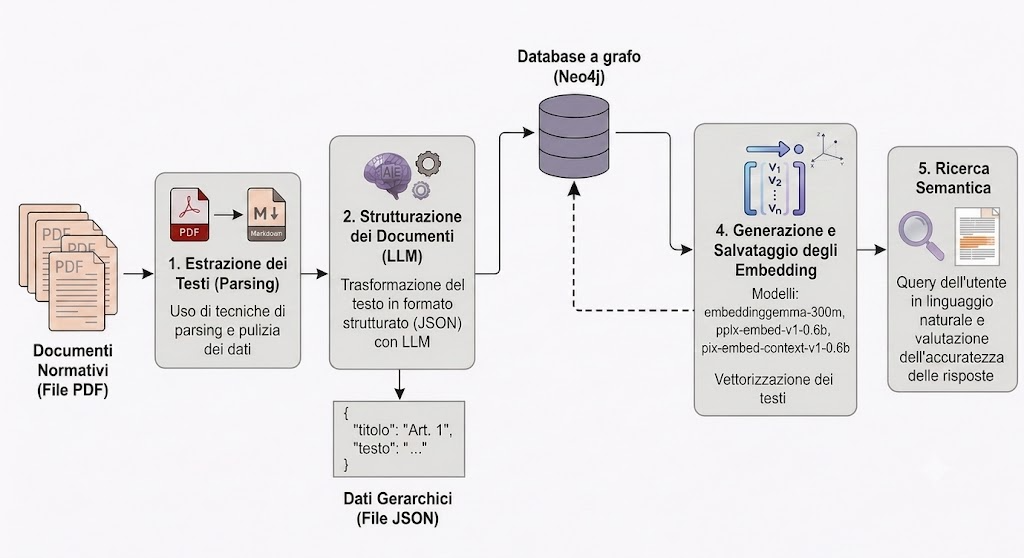
\includegraphics[width=1\textwidth]{_images/architettura-software.png}
    \caption{Architettura del sistema}
    \label{fig:architettura-software}
\end{figure}
    \chapter{Implementazione Software}\label{chap:fourth}

\inlineminitoc

In questo capitolo verranno analizzate nel dettaglio le singole fasi della pipeline di elaborazione, partendo dalle strategie di estrazione del testo grezzo, passando per la strutturazione semantica operata dai Large Language Models, fino ad arrivare alle logiche di ingestione e interrogazione sui database

\section{Estrazione dei Documenti}\label{sec:estrazione_documenti}
La fase iniziale della pipeline prevede l'estrazione del testo dai documenti normativi in formato PDF. 

Nelle prime fasi di sviluppo del progetto, l'intero documento PDF veniva passato direttamente al Large Language Model, demandando a quest'ultimo sia il compito di estrazione del testo grezzo sia quello di strutturazione sintattica. Questo approccio presentava forti criticità, esponeva il sistema al rischio di allucinazioni ed era inefficiente nel parsing di strutture complesse. Per superare tali limitazioni, la pipeline è stata modificata separando nettamente l'estrazione del testo dalla sua successiva strutturazione.

\subsection{Open Data Loader e la Gestione dei Tagged PDF}

Per l'estrazione del testo da documenti digitali nativi è stata adottata la libreria open-source \textit{Open Data Loader}. Questo strumento converte localmente i file PDF in formati ottimizzati per i LLM, specificamente Markdown. Il vantaggio di questa soluzione risiede nella sua natura deterministica: a parità di input viene garantito il medesimo output, azzerando le variabilità tipiche dei modelli generativi.

Durante l'analisi dei documenti legali, una delle criticità maggiori riguarda i ritorni a capo spuri, generati per ragioni puramente stilistiche (ad esempio, il raggiungimento del margine della pagina). Se non gestiti correttamente, questi si traducono in doppi ritorni a capo nel testo Markdown finale, frammentando artificialmente i periodi e compromettendo la qualità della successiva fase di chunking. Per risolvere questa criticità alla radice, l'estrazione è stata configurata abilitando il parametro specifico \texttt{use\_struct\_tree=True}.

Quando questo parametro è attivo, la libreria modifica il suo approccio di lettura, verificando innanzitutto se il file analizzato appartiene alla categoria dei \textit{Tagged PDF}. A differenza dei PDF standard, che definiscono esclusivamente il layout bidimensionale e visivo, i Tagged PDF incorporano un livello gerarchico logico e invisibile: il \textit{Logical Structure Tree}. Questo albero organizza il contenuto tramite elementi strutturali del tutto simili ai tag HTML (come \texttt{<H1>}, \texttt{<P>}, \texttt{<Table>}, \texttt{<L>}). 

Di conseguenza, abilitando \texttt{use\_struct\_tree=True}, \textit{Open Data Loader} è in grado di ignorare le fallaci euristiche geometriche e navigare direttamente la struttura logica del documento. Questo meccanismo permette all'estrattore di mappare ogni porzione di testo discriminando con precisione assoluta i semplici a capo visivi dalle reali interruzioni di paragrafo, restituendo un flusso di testo continuo e fedele all'originale.

Nel contesto della pubblica amministrazione, la formazione di documenti digitali adeguatamente strutturati non costituisce soltanto un'esigenza tecnica. L’articolo 40, comma 1, del Codice dell’Amministrazione Digitale (Decreto Legislativo 7 marzo 2005, n. 82), stabilisce infatti che \textquote{le pubbliche amministrazioni formano gli originali dei propri documenti [...] con mezzi informatici} \cite{cad_art40}.

Le modalità di formazione e gestione di tali documenti sono ulteriormente disciplinate dalle \textit{Linee guida sulla formazione, gestione e conservazione dei documenti informatici}, emanate dall'Agenzia per l'Italia Digitale ai sensi dell'articolo 71 del CAD \cite{agid_documenti_informatici}. In particolare, l'Allegato 2, dedicato ai formati di file, raccomanda di privilegiare formati \textquote{aperti, non proprietari, standard de iure, estendibili, parlanti, completamente robusti, indipendenti dal dispositivo} \cite{agid_formati_file}. Tali caratteristiche favoriscono l'interoperabilità, la conservazione nel tempo e il trattamento automatico dei documenti.

Nel caso dei file PDF, una struttura logica correttamente definita consente di rappresentare l'ordine di lettura e il ruolo semantico di elementi quali titoli, paragrafi, elenchi e tabelle. Quando presente, il \textit{Logical Structure Tree} costituisce inoltre per la pipeline sviluppata una fonte di informazioni pre-strutturate, utilizzabile per ricostruire con maggiore precisione la gerarchia e la sequenza logica del contenuto.


\subsection{Docling e l'Integrazione dei Motori OCR}

L'approccio standard basato su Open Data Loader mostra evidenti limiti in presenza di documenti non strutturati, con layout complessi o derivanti da scansioni visive, in quanto tale libreria non integra nativamente alcun modulo OCR. Per sopperire a questa mancanza è stata introdotta nel sistema la libreria \textit{Docling}. 

A differenza di Open Data Loader, Docling supporta l'integrazione diretta di motori OCR, configurandosi come un sistema avanzato di parsing e analisi del layout. Questo strumento, specializzato nell'estrazione di metadati, tabelle e testo da formati eterogenei, è stato quindi affiancato a Open Data Loader all'interno della pipeline, intervenendo come supporto specifico per processare tutti quei documenti in cui la sola estrazione con Open Data Loader risulta impossibile o inefficace.

L'introduzione dell'OCR ha sollevato complessità non trascurabili relative alla gestione delle risorse hardware all'interno dell'architettura a container. Il container Docker deputato all'estrazione operava infatti in condizioni in cui non poteva sprecare troppa RAM, date le risorse hardware limitate. Durante i primi test, l'invio massivo di interi documenti scansionati causava la saturazione istantanea della memoria, provocando l'intervento del modulo del kernel Linux (\textit{Out-Of-Memory Killer}) che terminava forzatamente il container.

Per superare il problema del consumo di RAM e prevenire i crash di sistema, è stata implementata una strategia basata sull'elaborazione pagina-per-pagina. Come discusso nel Capitolo \ref{chap:second} relativo alle scelte tecnologiche, a seguito di un'analisi comparativa dei motori supportati da Docling, la scelta è ricaduta su \textbf{RapidOCR}. Questo motore ha permesso di mantenere il consumo di memoria adeguato per il funzionamento del container, garantendo l'accuratezza del riconoscimento sul testo legale italiano.

\subsection{Progettazione del Custom Triage Processor}
Il processore di triage nativo di Open Data Loader prevede un flusso standard in cui ogni pagina viene analizzata e smistata: le pagine semplici vengono processate tramite il processo di Open Data Loader (una JVM), mentre le pagine complesse vengono delegate al backend basato su Docling. 

Tuttavia, l'applicazione con l'uso del parametro \texttt{use\_struct\_tree=True} introduce un bug logico nel triage di default: i documenti non espressamente \textit{tagged} vengono forzati all'interno del processo standard di Open Data Loader, non venendo mai instradati verso il backend di Docling, escludendo così l'analisi per pagine troppo complesse oppure l'attivazione dell'OCR dove necessario.

Per risolvere questa problematica è stato progettato e implementato un \textbf{Custom Triage Processor}. Come illustrato nel diagramma di flusso in \textbf{Figura \ref{fig:triage-processor}}, il componente corregge le anomalie di instradamento agendo secondo una logica a tre fasi:

\begin{itemize}
    \item \textbf{Fase 1: Verifica preliminare della struttura.} 
    Il file PDF viene acquisito e il sistema ne analizza i metadati per verificare se è codificato come \textit{Tagged PDF}. In caso affermativo, l'intero documento viene elaborato direttamente da Open Data Loader sfruttando l'albero strutturale nativo. Questo approccio garantisce la massima velocità di esecuzione e una pulizia ottimale del testo estratto.
    
    \item \textbf{Fase 2: Frazionamento del documento e stima della complessità.} 
    Se il documento risulta privo di struttura (\textit{Non-Tagged}), il flusso prevede la divisione in singole pagine indipendenti. Questa separazione è fondamentale per prevenire sovraccarichi di memoria RAM durante le elaborazioni successive. Per ciascuna pagina, il sistema calcola poi la densità dei caratteri testuali per valutarne il grado di complessità.
    
    \item \textbf{Fase 3: Triage ed elaborazione mirata della pagina.} 
    Sulla base dell'analisi precedente, ogni singola pagina subisce il processo di smistamento intelligente mostrato nella parte inferiore della Figura \ref{fig:triage-processor}, venendo indirizzata allo strumento di estrazione più adeguato:
    \begin{itemize}
        \item Se la pagina presenta un layout lineare e un'elevata densità di testo nativo, viene classificata come \textit{Semplice} e affidata al processo di Open Data Loader.
        \item Se la pagina contiene elementi geometrici articolati o tabelle annidate, ma il testo rimane comunque selezionabile, viene classificata come \textit{Complessa} e processata tramite Docling Standard (senza abilitare l'OCR).
        \item Se la pagina è priva di testo nativo (es. una fotocopia), viene classificata come \textit{Scansione} e inviata al container specializzato di Docling, dove interviene il motore RapidOCR per il riconoscimento ottico dei caratteri.
    \end{itemize}
\end{itemize}

\begin{figure}[H]
    \centering
    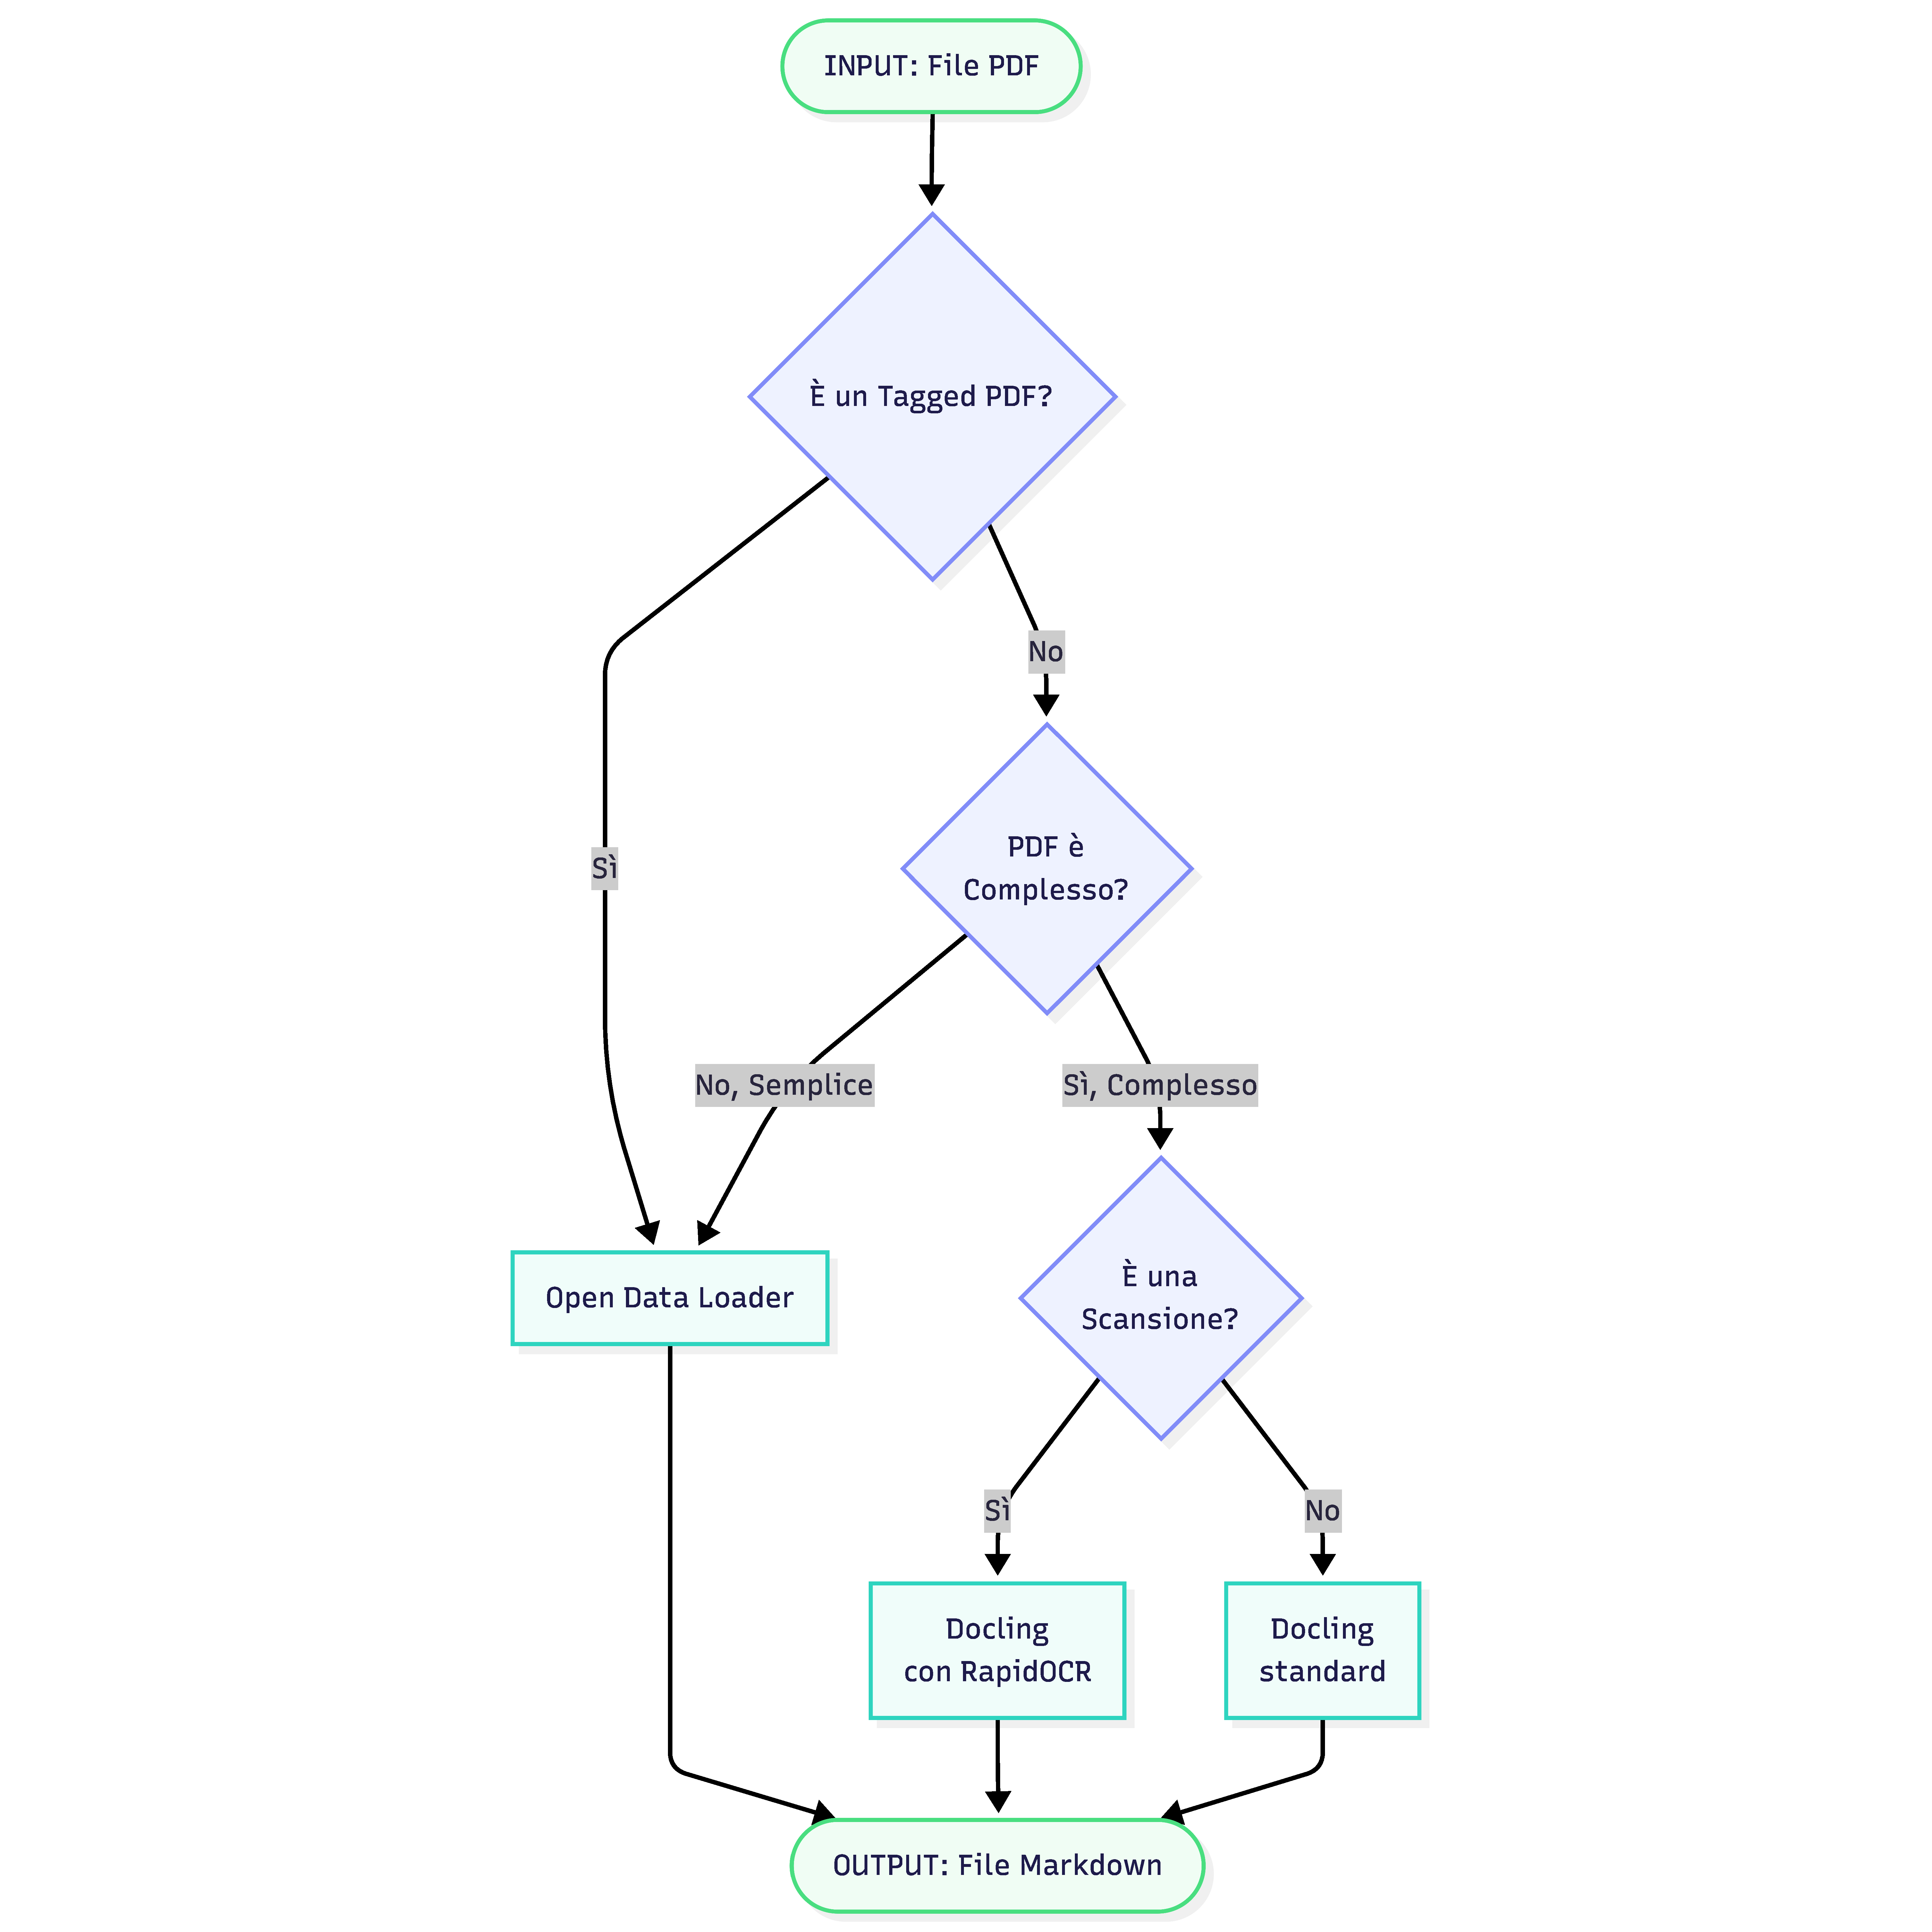
\includegraphics[width=1\textwidth]{_images/triage-processor.pdf}
    \caption{Flowchart del Custom Triage Processor}
    \label{fig:triage-processor}
\end{figure}
\newpage


\section{Strutturazione dei Documenti tramite LLM}
\label{sec:strutturazione_semantica}

Una volta ultimata la fase di estrazione del testo grezzo, illustrata nella sezione precedente, i documenti normativi si presentano sotto forma di file testuali piatti in formato Markdown. Tali file, pur contenendo l'intero testo originale, sono del tutto privi di metadati strutturali e di una formattazione gerarchica chiara. 
Poiché l'architettura di sistema prevede l'ingestione di questi documenti all'interno di un database a grafo (Neo4j) e in un database vettoriale (Qdrant), risulta indispensabile trasformare il testo non strutturato in una gerarchia rigorosa. L'archiviazione del solo testo grezzo, infatti, risulterebbe del tutto inadeguata e priva di utilità pratica. Una strutturazione accurata rappresenta il prerequisito fondamentale per abilitare qualsiasi operazione avanzata di \textit{information retrieval}, garantendo che i dati possano essere interrogati in modo efficiente e contestuale.

\subsection{Il Modello e la Strategia di Generazione}

Per affrontare il compito cruciale della strutturazione sintattica, è stato impiegato il Large Language Model \texttt{Gemini 3.5 Flash}. A livello di architettura software, il processo è diviso in due step distinti: la generazione di una struttura JSON gerarchica e l'estrazione delle relazioni semantiche tra le entità legali.

\subsection{Generazione della Struttura Gerarchica}

L'efficacia e l'accuratezza del processo di strutturazione si fondano su un \textit{System Prompt} ingegnerizzato ad hoc. Il suo compito principale è quello di mappare il contenuto all'interno del seguente schema logico:

\begin{itemize}
    \item \textbf{Metadati (\texttt{metadata}):} Il modello estrae e categorizza i dati identificativi dell'atto. Vengono isolati campi chiave come la data di stipula, il titolo completo e il nome del file originale.
    \item \textbf{Sezioni Introduttive e Conclusive:} Vengono separate dal corpo normativo tutte le sezioni di contorno. Tra queste figurano le premesse iniziali e le epigrafi (\texttt{preface}), gli indici (\texttt{preamble}), le dichiarazioni di chiusura con le relative firme (\texttt{conclusions}) e gli eventuali documenti annessi (\texttt{attachments}).
    \item \textbf{Corpo del Documento (\texttt{body}):} Rappresenta il nucleo dell'algoritmo di strutturazione. Il modello deve nidificare il testo seguendo fedelmente la gerarchia complessa e rigida tipica degli atti normativi italiani: \textbf{Titoli $>$ Capi $>$ Articoli $>$ Commi}.
\end{itemize}

Per garantire la massima coerenza dei dati all'interno del Knowledge Graph, sono state imposte al LLM regole tassative di parsing:

\begin{itemize}
    \item \textbf{Normalizzazione Numerica:} Tutti gli identificativi gerarchici originariamente espressi in numeri romani o in forma testuale (es. ``TITOLO I'', ``CAPO IV'') devono essere categoricamente convertiti in numeri interi arabi (1, 4, ecc.).
    \item \textbf{Gestione Dinamica dei Commi:} Poiché nei testi di legge i commi non sono sempre esplicitamente numerati, il modello è istruito a dedurli analizzando le interruzioni logiche dei paragrafi, assegnando loro una numerazione progressiva.
    \item \textbf{Ottimizzazione dello Schema:} Per mantenere leggeri i file JSON, il modello è programmato per non inizializzare chiavi con valori vuoti o nulli; se un livello gerarchico (come un Capo o un Titolo) non trova riscontro nel testo originale, la proprietà viene semplicemente omessa.
\end{itemize}

L'esecuzione di questo processo restituisce una directory di documenti JSON puliti e strutturati gerarchicamente, pronti per essere archiviati e per affrontare il successivo step: l'estrazione delle relazioni semantiche tra le entità legali.

\subsection{Estrazione delle Relazioni Semantiche}

La sola scomposizione del testo normativo in una struttura gerarchica ad albero rappresenta una condizione necessaria ma non sufficiente per la costruzione di un vero e proprio \textit{Knowledge Graph}. Per sfruttare appieno la potenza topologica di un database a grafo come Neo4j, è indispensabile individuare e mappare esplicitamente i collegamenti e le dipendenze logiche che intercorrono tra le diverse disposizioni giuridiche all'interno dello stesso atto. A questo scopo, la pipeline prevede un secondo step logico interamente dedicato all'estrazione delle relazioni semantiche.
In questa fase, l'input non è più il testo grezzo, ma i file JSON prodotti nello step precedente, che quindi agiscono come una base di conoscenza consolidata. Ciascun documento viene quindi analizzato dal LLM \texttt{Gemini 3.5 Flash}, guidato da un \textit{System Prompt} specializzato. Tale prompt è stato progettato per riconoscere i costrutti linguistici del gergo giuridico che indicano un collegamento formale tra le parti del testo. Le relazioni estratte sono:
\begin{itemize}
    \item \textbf{CITA:} Un articolo o comma fa riferimento a un'altra disposizione.
    \item \textbf{ABROGA:} Una disposizione annulla la validità giuridica di un'altra.
    \item \textbf{DEROGA:} Un elemento introduce un'eccezione a una regola generale.
    \item \textbf{SOSTITUISCE:} Una disposizione prende il posto di un'altra.
    \item \textbf{INTERPRETA:} La comprensione di una norma dipende dalla lettura di un'altra.
\end{itemize}

L'output di questa analisi è una rete di collegamenti formali, dove per ciascuna relazione vengono specificati il nodo di partenza, il nodo di arrivo e il tipo di legame. Queste informazioni sono esportate in un nuovo set di file JSON.

Questo approccio a due stadi permette di separare le responsabilità e ridurre il carico cognitivo del modello a ogni ciclo. In questo modo si produce un dataset pulito e affidabile, pronto per essere caricato nel grafo.

\section{Importazione dati nei Database}
\label{sec:database_ingestion}

Una volta completata la strutturazione dei documenti legali in formato JSON, si apre la fase di persistenza e indicizzazione dei dati. Nel contesto di questo progetto di tirocinio, l'architettura prevede il caricamento dei dati estratti all'interno del database a grafo Neo4j.

Per garantire la flessibilità e favorire un ambiente di sviluppo pulito e modulare, lo sviluppo del software ha visto l'applicazione del \textit{Repository Pattern} e l'uso di interfacce polimorfiche.

\subsection{I Modelli di Dominio}
\label{sec:modelli_dominio}
Prima di analizzare le strategie di persistenza, è fondamentale descrivere come i dati estratti vengano rappresentati. All'interno della cartella \texttt{models} di questo step, il sistema definisce le entità fondamentali del dominio normativo utilizzando il paradigma ad oggetti. Queste classi operano essenzialmente come \textit{Entities}: strutture dati pure, prive di logica di persistenza diretta o dipendenze verso i DBMS, il cui unico scopo è incapsulare i dati del dominio.

L'architettura dei modelli è rappresentata nel diagramma UML della Figura \ref{fig:domain-models-class-diagram}. Le principali classi sono:
\begin{itemize}
    \item \texttt{Entity}: Incapsula l'ente pubblico emittente, memorizzando i metadati di dominio.
    \item \texttt{LegalAct}: È la classe orchestratrice principale. Rappresenta l'atto legale nella sua interezza e contiene i metadati principali (title, publication\_date, file\_name) e soprattutto una lista \texttt{elements} che tiene traccia di tutti i sotto-elementi istanziati e delle loro relazioni gerarchiche.
    \item \texttt{StructuralElement}: È la classe base polimorfica per mappare le sottoclassi \texttt{Title}, \texttt{Chapter} e \texttt{Article}, mantenendo traccia del numero d'ordine e dell'eventuale rubrica.
    \item \texttt{Paragraph}: Rappresenta il comma ed è l'unità atomica d'informazione sulla quale verranno calcolati gli embedding.
\end{itemize}

\begin{figure}[H]
    \centering
    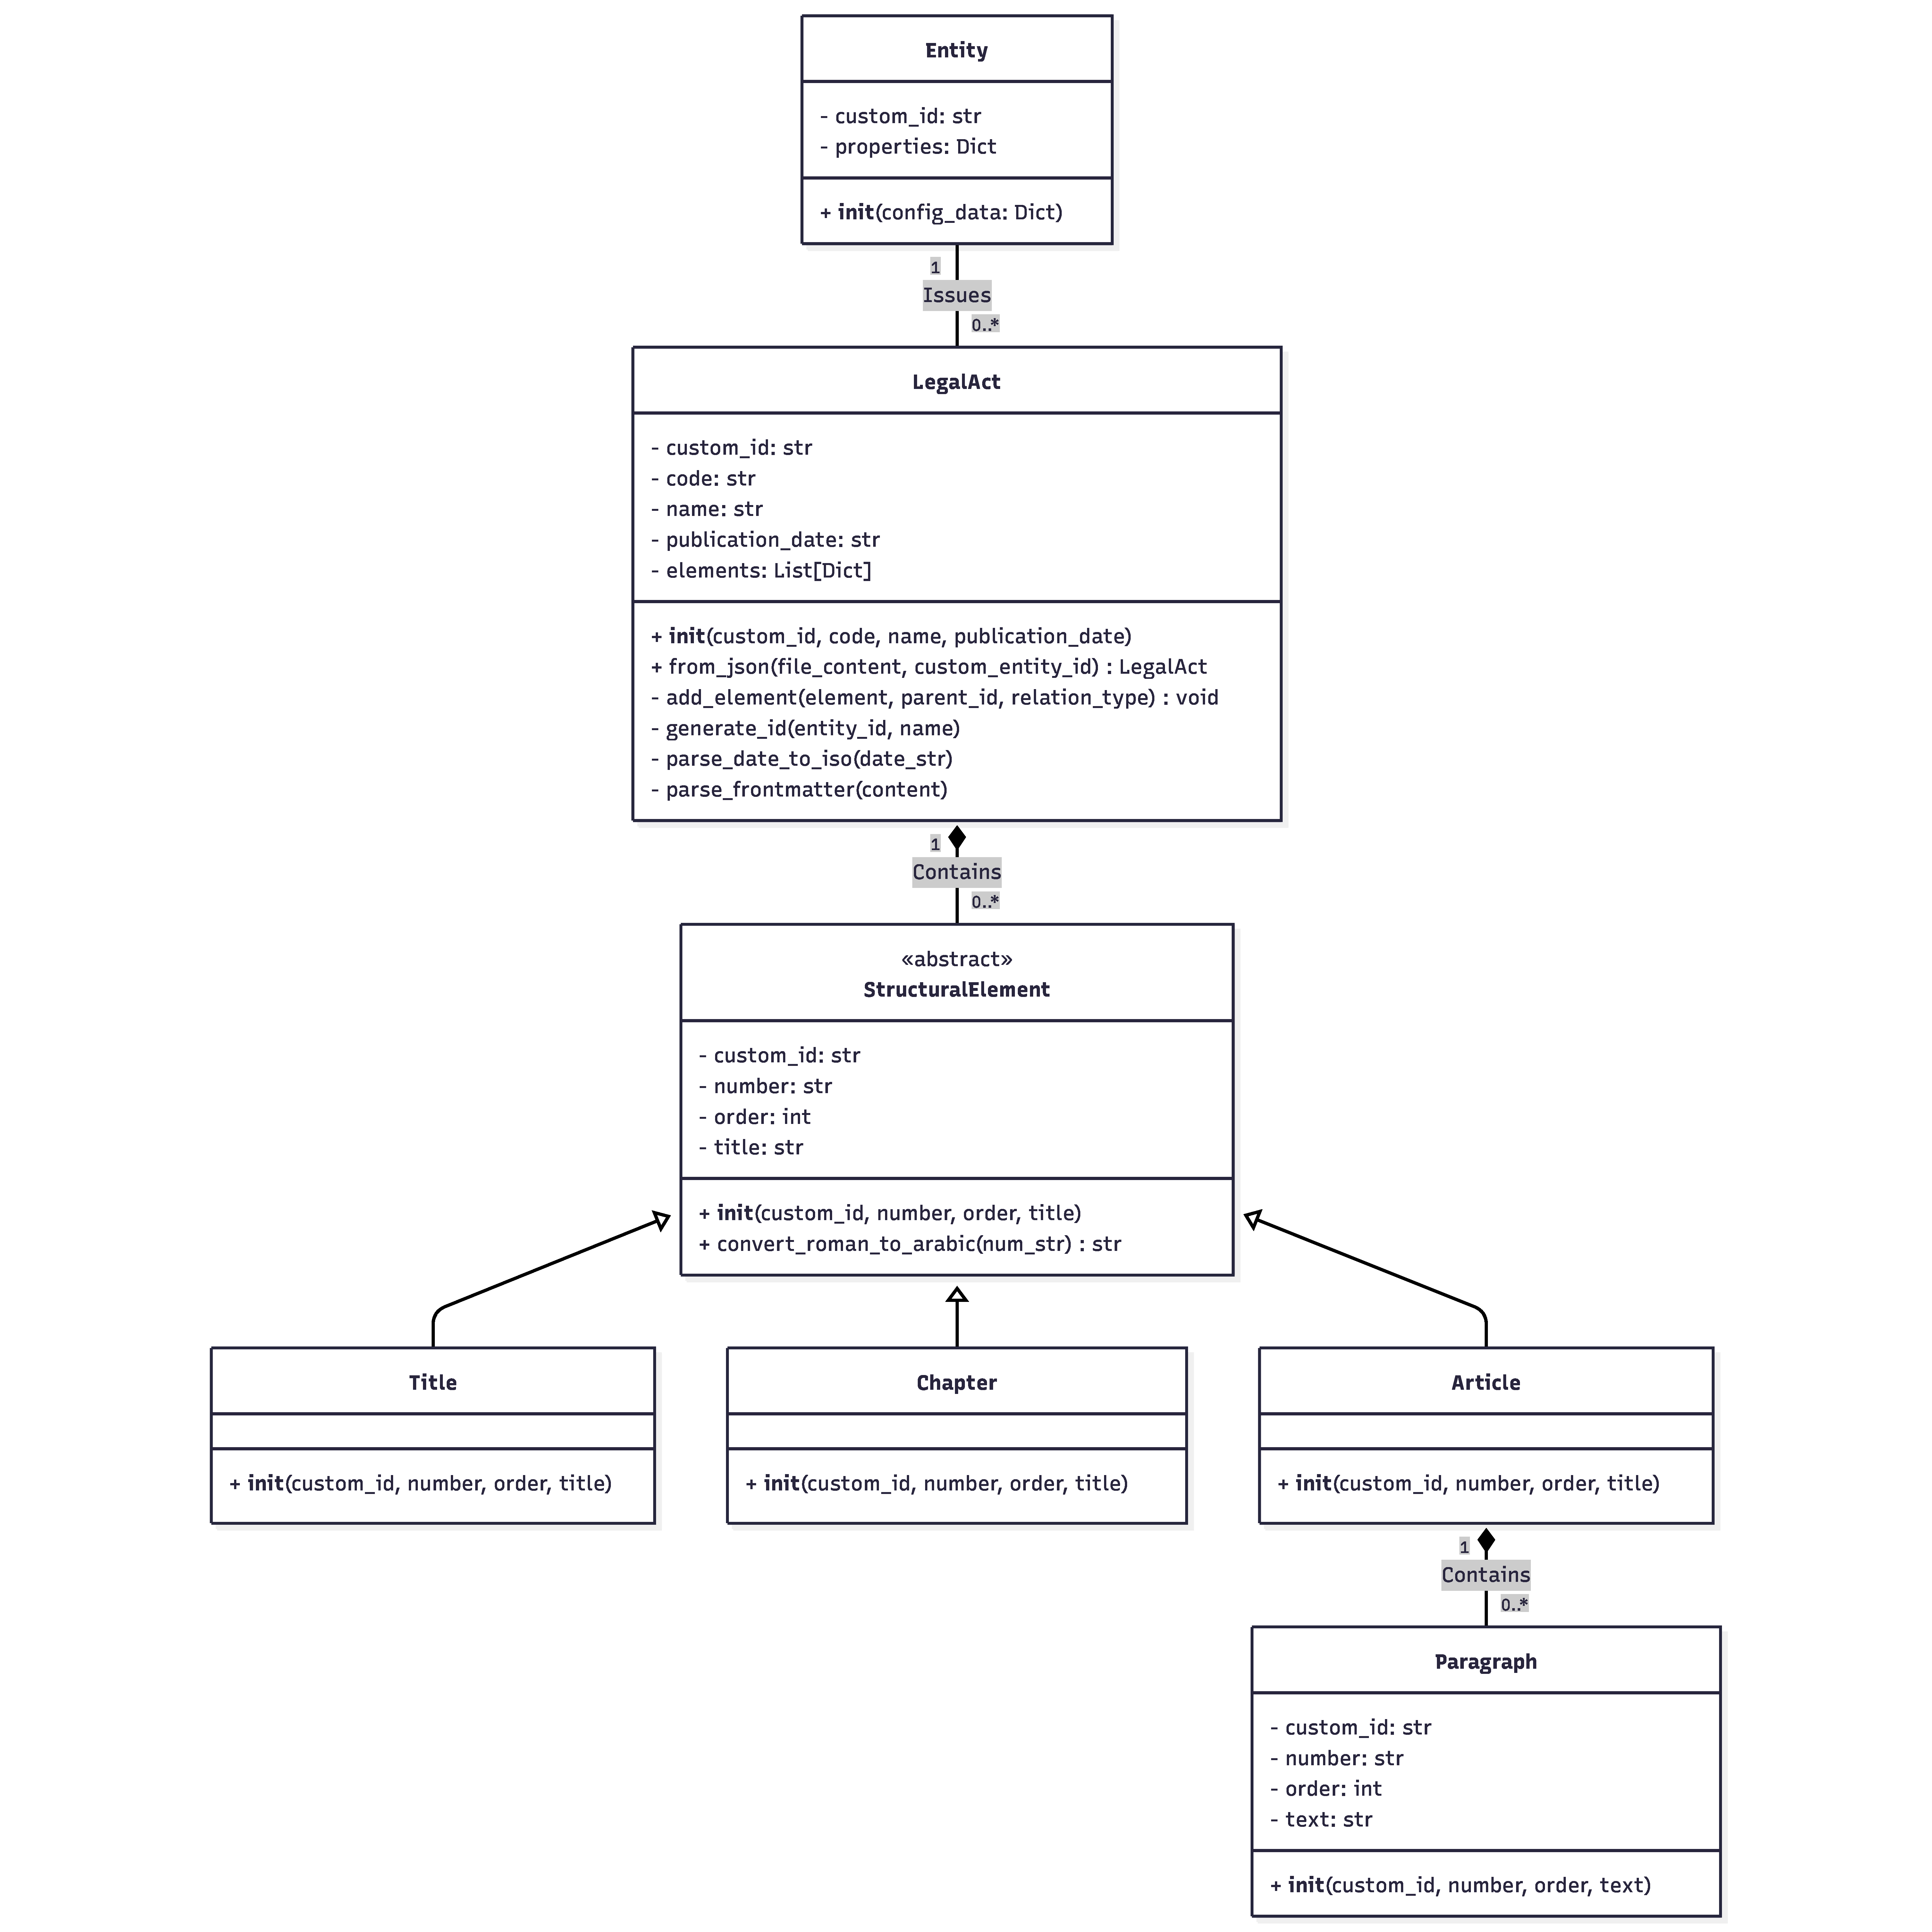
\includegraphics[width=1\textwidth]{_images/domain-models-class-diagram.pdf}
    \caption{Class Diagram dei modelli di dominio}
    \label{fig:domain-models-class-diagram}
\end{figure}


\subsection{Interfaccia per il disaccoppiamento della persistenza}
L'adozione di un'interfaccia comune di importazione nasce dalla precisa volontà di disaccoppiare la logica di lettura dei dati dalla loro effettiva persistenza fisica.
Sebbene l'attuale implementazione preveda l'utilizzo esclusivo del database a grafo Neo4j, questa scelta architetturale si rivela strategica per sviluppi futuri. Qualora si rendesse necessario integrare nuovi DBMS (ad esempio, un database puramente vettoriale dedicato esclusivamente agli embedding), sarà sufficiente implementare una nuova classe concreta senza dover alterare il flusso principale del programma. Inoltre, il disaccoppiamento garantisce un'elevata testabilità del codice, permettendo di validare la logica di dominio e il parsing dei documenti simulando le operazioni di salvataggio indipendentemente dal database sottostante.

Nel sistema sviluppato, l'interfaccia astratta di riferimento è rappresentata dalla classe \texttt{DBImporterInterface}. Essa definisce tre metodi fondamentali che ogni classe concreta deve implementare:
\begin{itemize}
    \item \texttt{connect()}: per la gestione e la validazione della connessione con l'istanza specifica del database;
    \item \texttt{import\_legal\_act(entity, legal\_act)}: per l'esecuzione effettiva di ingestion dell'atto normativo e dell'ente emittente;
    \item \texttt{close()}: per la chiusura sicura delle sessioni.
\end{itemize}


\subsection{Architettura del Database Neo4j}
\label{subsec:neo4j_architecture}

Il database modella fedelmente l'albero gerarchico discendente del documento, garantendo la flessibilità necessaria per gestire percorsi diretti qualora i livelli intermedi siano stati omessi durante la strutturazione JSON (es. \texttt{LegalAct $\rightarrow$ Article $\rightarrow$ Paragraph}). 

Le \textit{Label} dei nodi sul grafo (ovvero \textbf{Entity}, \textbf{LegalAct}, \textbf{Title}, \textbf{Chapter}, \textbf{Article} e \textbf{Paragraph}) riflettono rigorosamente la struttura delle classi di dominio già presentate nella Sezione \ref{sec:modelli_dominio}, così proprio come le \textit{Properties} dei nodi, che conservano i metadati principali e le informazioni testuali.

Un aspetto architetturale chiave, comune a tutti i nodi, è la presenza della proprietà \texttt{custom\_id}. Tale attributo codifica per intero il percorso gerarchico del nodo all'interno del documento (ad esempio, \texttt{ente\_\_atto\_\_title-1\_\_chapter-2\_\_article-3\_\_paragraph-4}). Grazie a questo approccio, il database può sfruttare l'indicizzazione su questa proprietà per individuare immediatamente un singolo nodo, azzerando le operazioni di attraversamento del grafo e garantendo un recupero delle informazioni in tempo costante.

All'interno di questa topologia, i nodi di tipo \textbf{Paragraph} ricoprono un ruolo centrale per le funzionalità avanzate del sistema. Oltre a conservare le proprietà testuali, in questi nodi vengono salvate le rappresentazioni vettoriali dei dati: in particolare, gli embedding semantici a dimensione variabile e un embedding strutturale a 128 dimensioni calcolato mediante l'algoritmo di \textit{Node2Vec} (maggiori informazioni sono nel capitolo \ref{sec:creazione_embedding}). L'archiviazione di tali vettori è progettata per abilitare le successive operazioni di interrogazione.

L'ecosistema di relazioni (\textit{Edges}) all'interno del grafo si articola in tre macro-categorie progettate per supportare le interrogazioni avanzate:
\begin{itemize}
    \item \textbf{Relazioni Strutturali}: Definiscono la topologia discendente del documento normativo. Comprendono l'arco \texttt{ISSUES} che lega l'Ente all'Atto, e la catena di contenimento gerarchico formata da \texttt{HAS\_TITLE}, \texttt{HAS\_CHAPTER}, \texttt{HAS\_ARTICLE} e \texttt{HAS\_PARAGRAPH}.
    \item \textbf{Relazioni Sequenziali}: I commi appartenenti allo stesso articolo sono concatenati linearmente tramite la relazione \texttt{NEXT\_PARAGRAPH}. Questa architettura a lista concatenata si rivela fondamentale per espandere dinamicamente la finestra di contesto durante la fase di interrogazione, permettendo di recuperare i commi logicamente antecedenti o successivi senza dover eseguire query computazionalmente costose per ricalcolare l'ordine strutturale.
    \item \textbf{Relazioni Legali}: Traducono in archi orientati sul grafo i collegamenti logici e giuridici intra-documento individuati dal prompt specializzato dell'LLM (Sezione \ref{sec:strutturazione_semantica}). Le cinque tipologie di relazione estratte vengono trasposte fedelmente nelle label \texttt{CITES}, \texttt{REPEALS}, \texttt{INTERPRETS}, \texttt{REPLACES} e \texttt{DEROGATES}. 
\end{itemize}

Occorre precisare che, sebbene lo schema dati supporti nativamente tutte le interazioni legali sopracitate, l'attuale popolamento del database non registra occorrenze per le relazioni \texttt{REPEALS} e \texttt{REPLACES}. Questa mancanza non è imputabile a un difetto del sistema di estrazione, bensì rappresenta un limite intrinseco dei documenti elaborati, che non contengono clausole esplicite di abrogazione o sostituzione strutturata.

\subsection{Dettagli Implementativi dell'Ingestion su Neo4j}
Un atto legale non può essere salvato tramite un'unica operazione atomica standard, a causa delle complesse connessioni tra i nodi, per questo motivo la responsabilità è stata distribuita su una serie di repository specializzati, ognuno deputato alla gestione del ciclo di vita di un singolo modello di dominio:
\begin{itemize}
    \item \texttt{EntityRepository}: Gestisce l'inserimento dei nodi relativi agli enti istituzionali.
    \item \texttt{LegalActRepository}: Inserisce il nodo radice dell'atto e lo ancora all'ente emittente.
    \item \texttt{StructuralElementRepository}: Incapsula la logica Cypher necessaria a creare i nodi intermedi del grafo e gli archi verso i rispettivi nodi padri.
    \item \texttt{ParagraphRepository}: Si occupa esclusivamente della persistenza dei nodi foglia contenenti il testo dei commi.
\end{itemize}

Per quanto riguarda il salvataggio delle relazioni trasversali, queste informazioni vengono lette da file JSON esterni dedicati (Sezione \ref{sec:estrazione_relazioni}), per poi essere elaborate da un metodo che, attraverso i \texttt{custom\_id} dei nodi salvati e indicizzati sul grafo, trova in maniera quasi istantanea i nodi correlati dall'estratto JSON ed esegue una query Cypher dedicata per la creazione dell'arco semantico.

\begin{lstlisting}[language=Cypher, caption={Query Cypher per l'inserimento delle relazioni legali}, label={lst:cypher_relationships}]
MATCH (s {custom_id: $source_id})
WITH s
MATCH (t {custom_id: $target_id})
MERGE (s)-[r:`<rel_type>`]->(t)
RETURN r
\end{lstlisting}

\noindent L'obiettivo di questa query è rintracciare i due nodi di interesse (sorgente e destinazione) tramite il loro identificativo univoco e stabilire una relazione orientata tra di essi.

Di seguito troviamo un esempio di relazione estratta in formato JSON, con ID parzialmente omessi per motivi di leggibilità:

\begin{lstlisting}[caption={Esempio reale di relazione estratta in formato JSON}, label={lst:json-cites}, breaklines=true]
{
  "sourceId": "ente-provincia-taranto__contratto-collettivo-[...]__title-2__chapter-2__article-8__paragraph-6",
  "relationshipType": "CITES",
  "targetId": "ente-provincia-taranto__contratto-collettivo-[...]__title-2__chapter-2__article-8__paragraph-1"
}
\end{lstlisting}

A supporto di quanto descritto, la Figura \ref{fig:relationship_example} fornisce una rappresentazione visiva delle relazioni instaurate tra i nodi dell'articolo 8 del seguente atto: \texttt{"CCNL del personale non dirigente del comparto regioni e autonomie locali"}

\begin{figure}[H]
    \centering
    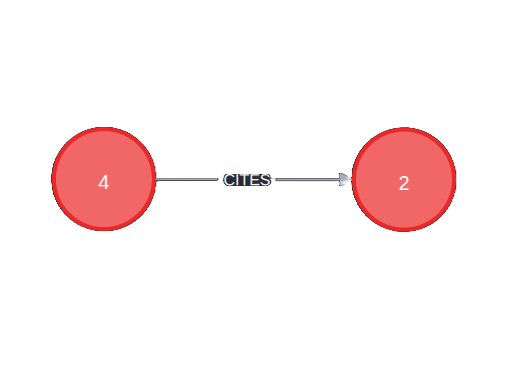
\includegraphics[width=1\textwidth]{_images/relationship.png}
    \caption{Rappresentazione visiva delle relazioni instaurate tra i nodi dell'articolo 8 di un atto normativo.}    
    \label{fig:relationship_example}
\end{figure}

\subsection{Risultati e Metriche}
L'esecuzione della pipeline di ingestion ha dimostrato un'elevata efficienza, completando il caricamento dell'intero dataset all'interno del database in un tempo complessivo di \textbf{50.29 secondi}.

Il processo ha popolato il grafo con un totale di 8.535 nodi e 14.201 relazioni. Di seguito viene riportato il dettaglio quantitativo delle entità di dominio e degli archi salvati.

La Tabella \ref{tab:statistiche_nodi} illustra la distribuzione dei nodi all'interno del grafo, raggruppati per \textit{Label}. Come si può osservare dai dati, vi è una netta preponderanza numerica dei nodi \texttt{Paragraph}, i quali rappresentano l'unità atomica d'informazione su cui si basano le successive operazioni di embedding e ricerca.

\begin{table}[H]
    \centering
    \renewcommand{\arraystretch}{1.2}
    \begin{tabular}{|l|r|}
        \hline
        \textbf{Label Nodo} & \textbf{Quantità} \\
        \hline
        \texttt{Paragraph} & 6.396 \\
        \texttt{Article} & 1.802 \\
        \texttt{Chapter} & 147 \\
        \texttt{LegalAct} & 95 \\
        \texttt{Title} & 93 \\
        \texttt{Entity} & 2 \\
        \hline
    \end{tabular}
    \caption{Statistica dei nodi inseriti nel database Neo4j.}
    \label{tab:statistiche_nodi}
\end{table}

Per quanto riguarda invece le interconnessioni tra le entità, la Tabella \ref{tab:statistiche_relazioni} dettaglia il conteggio esatto degli archi strutturali, sequenziali e legali creati durante l'importazione.

\begin{table}[H]
    \centering
    \renewcommand{\arraystretch}{1.2}
    \begin{tabular}{|l|r|}
        \hline
        \textbf{Tipo di Relazione} & \textbf{Quantità} \\
        \hline
        \texttt{HAS\_PARAGRAPH} & 6.396 \\
        \texttt{NEXT\_PARAGRAPH} & 4.594 \\
        \texttt{HAS\_ARTICLE} & 1.802 \\
        \texttt{CITES} & 1.030 \\
        \texttt{HAS\_CHAPTER} & 147 \\
        \texttt{ISSUES} & 95 \\
        \texttt{HAS\_TITLE} & 93 \\
        \texttt{DEROGATES} & 41 \\
        \texttt{INTERPRETS} & 3 \\
        \hline
    \end{tabular}
    \caption{Statistica delle relazioni inserite nel database Neo4j.}
    \label{tab:statistiche_relazioni}
\end{table}

Come si evince dalla Tabella \ref{tab:statistiche_relazioni}, l'analisi degli archi conferma la solidità dell'architettura a lista concatenata, evidenziata dal notevole volume di relazioni \texttt{NEXT\_PARAGRAPH} (4.594), essenziali per l'espansione dinamica del contesto in fase di retrieval. 

Inoltre, analizzando sempre i medesimi dati in merito agli archi logico-legali, si osserva una netta predominanza delle relazioni di citazione (\texttt{CITES}, 1.030 occorrenze), seguite da un numero minoritario di deroghe (\texttt{DEROGATES}, 41) e interpretazioni (\texttt{INTERPRETS}, 3). Coerentemente con quanto anticipato nella Sezione \ref{subsec:neo4j_architecture}, le metriche riportate confermano l'assenza totale di occorrenze per le relazioni di abrogazione (\texttt{REPEALS}) e sostituzione (\texttt{REPLACES}) all'interno di questo specifico bacino documentale.

\subsection{Visualizzazione del Grafo}
A conclusione di questo capitolo, si propone una rappresentazione visiva di un estratto del database Neo4j volta a mostrare in maniera intuitiva la topologia della rete. Nella Figura \ref{fig:graph-visualization} è possibile osservare la struttura gerarchica e le connessioni tra le diverse entità, evidenziate mediante una differenziazione cromatica:
\begin{itemize}
    \item I \textbf{nodi gialli} rappresentano l'ente emittente (\texttt{Entity});
    \item I \textbf{nodi azzurri} indicano gli atti legali (\texttt{LegalAct});
    \item I \textbf{nodi rossi} corrispondono ai commi (\texttt{Paragraph});
    \item I \textbf{restanti nodi} raffigurano le altre parti della gerarchia strutturale del documento, ossia i titoli (\texttt{Title}), i capi (\texttt{Chapter}) e gli articoli (\texttt{Article}).
\end{itemize}

\begin{figure}[H]
    \centering
    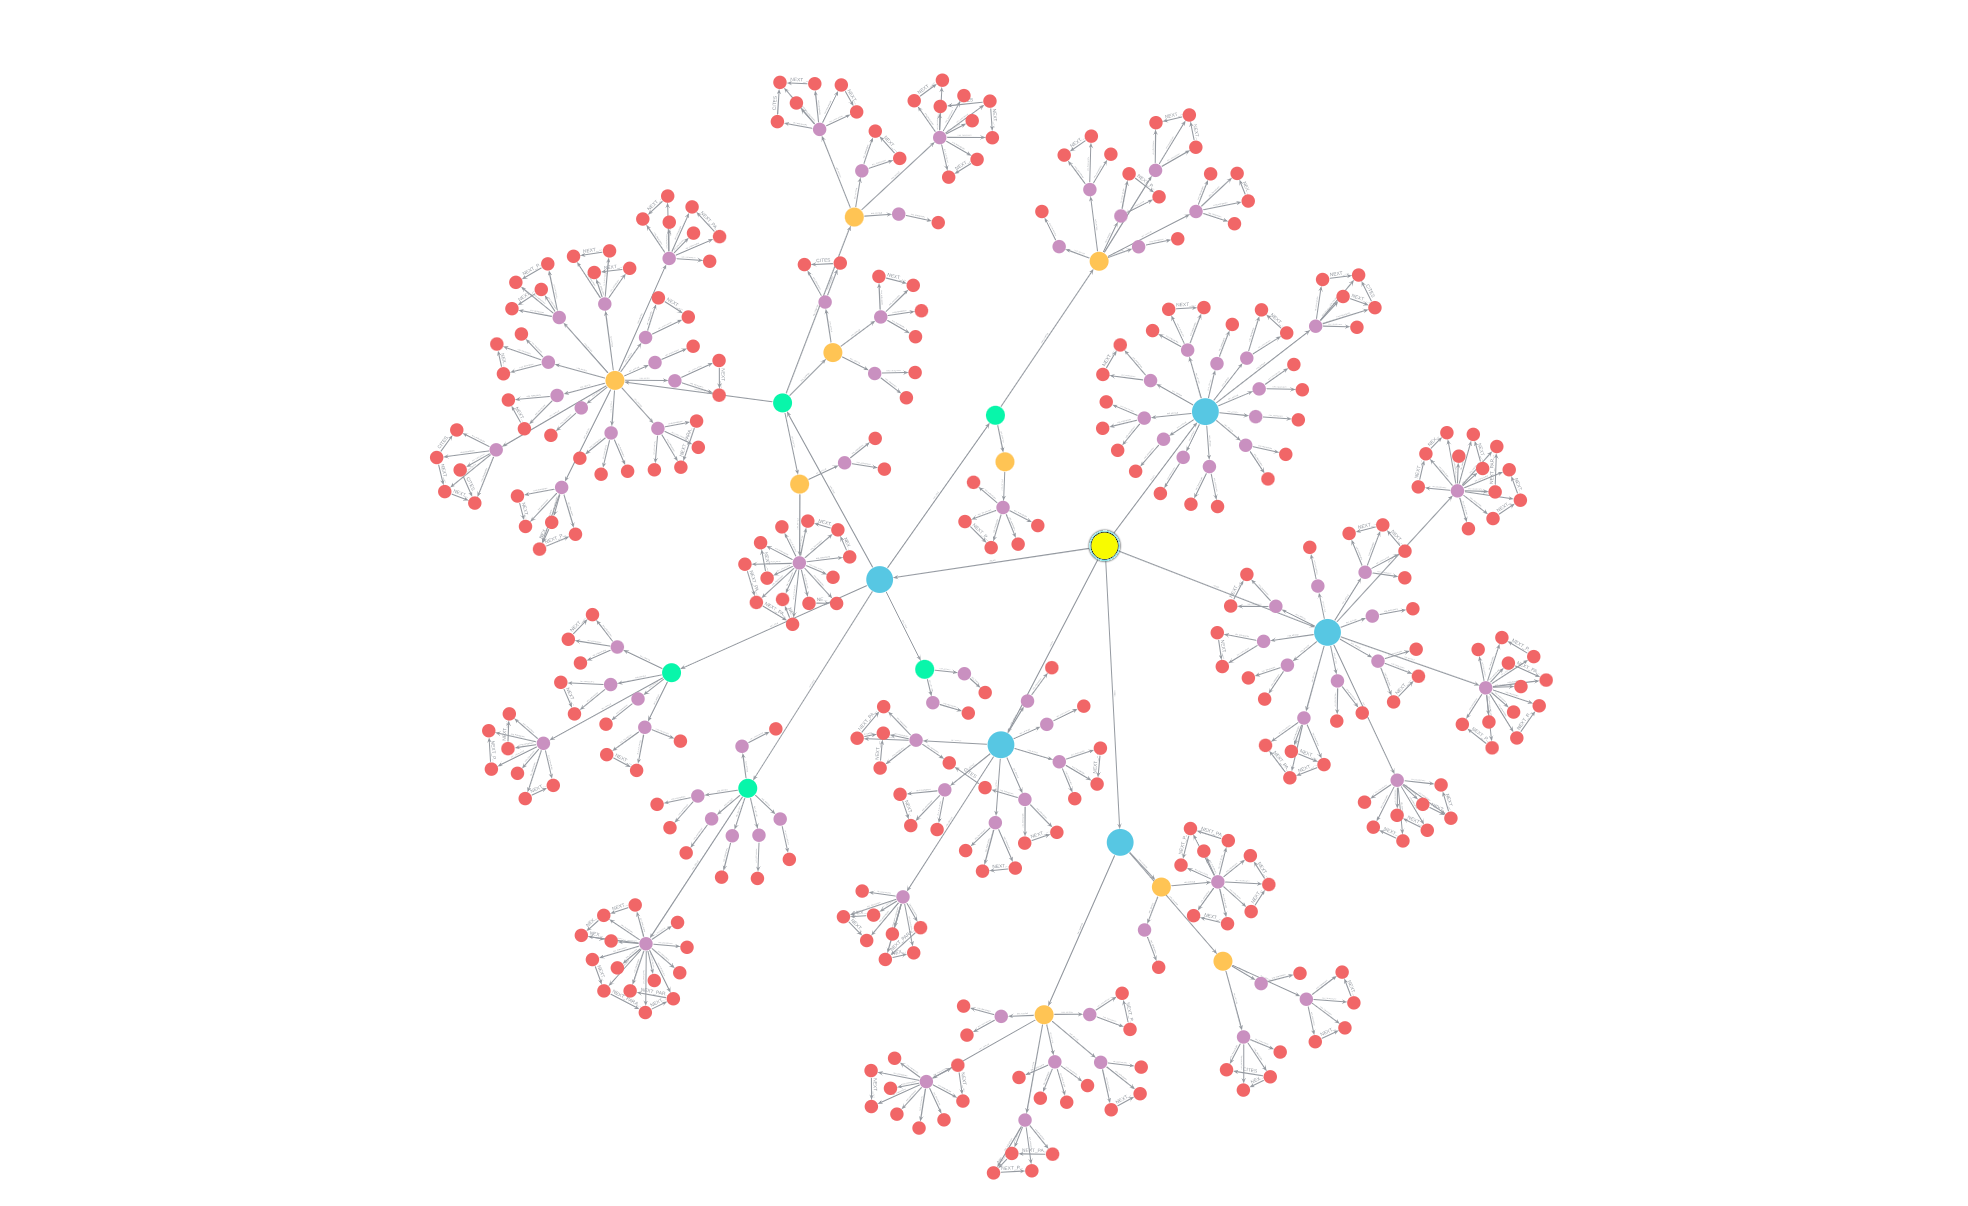
\includegraphics[width=1\textwidth]{_images/graph-visualization.png}
    \caption{Rappresentazione visiva di un estratto del database a grafo Neo4j.}
    \label{fig:graph-visualization}
\end{figure}

\newpage
\section{Creazione degli Embedding}
\label{sec:creazione_embedding}

L'operazione di vettorizzazione, o di \textit{embedding}, rappresenta un passaggio cruciale per abilitare le funzionalità di ricerca semantica all'interno del database a grafo.
La pipeline supporta tre modelli di embedding, dettagliati nella sezione \ref{sec:llm_embedding_models}: 
\begin{itemize}
    \item \texttt{google/embeddinggemma-300m}
    \item \texttt{perplexity-ai/pplx-embed-v1-0.6b}
    \item \texttt{perplexity-ai/pplx-embed-context-v1-0.6b}
\end{itemize}

I vettori vengono archiviati direttamente come proprietà all'interno dei nodi (\texttt{:Paragraph}) già esistenti nel grafo. Questo evita la necessità di un database vettoriale separato e consente al modello di ricerca di operare direttamente su Neo4j.

Neo4j, inoltre, supporta la creazione di indici vettoriali utilizzando algoritmi di ricerca approssimata (\textit{Approximate Nearest Neighbor Search}, ANN). Invece di calcolare la distanza coseno tra il vettore di query e tutti gli altri vettori (operazione $O(n)$ molto costosa), questi indici riducono drasticamente lo spazio di ricerca. Di conseguenza, il tempo di esecuzione delle query passa da secondi a millisecondi, rendendo la ricerca praticabile anche su documenti normativi di grandi volumi.

\subsection{Differenza nell'Arricchimento Contestuale: Standard vs Late Chunking}
\label{subsec:arricchimento_contestuale}
 
Il sistema implementa due approcci diversi per fornire \textit{contesto} ai commi. Se si fornisce al modello solo la stringa del comma \textquote{... è punito con la reclusione da 1 a 3 anni}, l'embedding generato risulterà limitato, poiché il testo manca di informazioni fondamentali come il soggetto e il reato specifico (elementi definiti nei livelli superiori come l'articolo o il titolo).
Ecco come le due metodologie risolvono il problema:
 
\subsubsection{A. Arricchimento Standard (Modelli: Gemma 300m e PPLX-v1)}
 
In questo approccio, il contesto viene iniettato testualmente attraverso \textit{String Concatenation}.
Per ciascun comma, viene recuperato il contesto gerarchico risalendo l'albero strutturale tramite query Cypher. Tutte queste informazioni vengono concatenate in un'unica stringa, producendo un testo inviato al modello simile al seguente:

\begin{center}
    \texttt{\textquote{Atto: Codice Penale | Titolo 3 Dei delitti contro l'amministrazione della giustizia | Capo 2 Dei delitti contro l'autorità delle decisioni giudiziarie | Art. 385 Evasione | Comma 1 | ... è punito con la reclusione da 1 a 3 anni.}}
\end{center}

In questo approccio, ogni comma viene trattato come un \textit{chunk isolato} al momento dell'embedding. Sebbene il modello riceva il testo arricchito dai metadati gerarchici, il contesto rimane limitato a questo preambolo testuale statico.
 
\subsubsection{B. Arricchimento tramite Late Chunking (Modello: PPLX-Context)}
 
Questo approccio impiega una vera e propria contestualizzazione a livello di rete neurale. A differenza dell'approccio standard, non utilizza preamboli testuali pre-calcolati, ma affida la comprensione semantica direttamente all'algoritmo di \textit{self-attention} del modello.

Il sistema recupera dal database, tramite query Cypher, l'intero articolo con tutti i commi che lo compongono, mantenendo traccia dell'ordine sequenziale e dei confini esatti tra di essi. Invece di frammentare il testo a monte e inviare al modello i commi singolarmente, il sistema li presenta all'encoder come un'unica sequenza di input ininterrotta.

È in questa fase che agisce il meccanismo di \textit{late chunking}. Il modello processa l'articolo nella sua interezza attraverso i successivi layer del Transformer; in questo modo, la \textit{self-attention} bidirezionale permette ai token di ciascun comma di "prestare attenzione" e interagire con i token adiacenti e con l'intero testo. Questo approccio abbatte i confini artificiali del chunking testuale, permettendo alla rete di risolvere dinamicamente pronomi, riferimenti incrociati e concetti impliciti basandosi sul contesto normativo globale.

Solo nella fase finale, dopo che ogni singolo token ha assorbito un significato profondamente contestualizzato, il modello applica un'operazione di \textit{pooling} differenziata. Sfruttando gli indici sequenziali salvati in precedenza, estrae e restituisce gli embeddings separati per ciascun comma originale. Questa architettura garantisce che l'embedding finale di un singolo comma racchiuda non solo il suo significato letterale, ma anche le sfumature semantiche derivanti dal resto dell'articolo, unendo la massima precisione granulare a una perfetta consapevolezza del contesto globale.

Un esempio pratico:

\begin{quote}
\texttt{Comma 1: "I soggetti che omettono la dichiarazione dei redditi sono puniti con una sanzione di 1.000 euro."}

\texttt{Comma 2: "La disposizione non si applica se essi dimostrano l'assenza di dolo."}
\end{quote}

Se il modello processa il Comma 2 in isolamento, la parola "essi" è ambigua e "La disposizione" è un concetto vuoto.
Sfruttando il late chunking, la rete neurale collega istantaneamente "essi" del Comma 2 ai "soggetti" del Comma 1, e "La disposizione" all'intero concetto di sanzione appena letto.

\subsection{Il Graph Embedding come appoggio agli Embedding Semantici}
Oltre all'analisi puramente testuale, il sistema arricchisce la rappresentazione della conoscenza integrando l'informazione strutturale del documento. A tale scopo viene impiegato l'algoritmo \textbf{Node2Vec}, eseguito tramite la libreria Graph Data Science (GDS). Questo approccio genera un \textit{graph embedding} per ogni comma, codificando in vettori a 128 dimensioni la topologia della rete, ovvero la gerarchia del documento e le relazioni logico-giuridiche che legano i nodi. In questo modo, l'algoritmo mappa in regioni vicine dello spazio vettoriale quei commi che, a prescindere dal testo, condividono una medesima posizione strutturale o forti vincoli normativi.
Per adattare Node2Vec al dominio legale, la strategia di esplorazione del grafo tramite \textit{random walk} è stata calibrata attraverso i parametri \textbf{p} e \textbf{q}:
\begin{itemize}
    \item \textbf{Return parameter ($p = 1$)}: Mantiene un comportamento esplorativo neutrale, senza forzare né penalizzare il ritorno immediato al nodo precedente.
    \item \textbf{In-out parameter ($q = 0.5$)}: Essendo inferiore a $1$, forza un'esplorazione profonda (simile a una \textit{Depth-First Search}). Questa scelta è essenziale nel dominio legale, in quanto permette all'algoritmo di attraversare in profondità l'intera struttura verticale del documento (Legge $\rightarrow$ Titolo $\rightarrow$ Capo $\rightarrow$ Articolo $\rightarrow$ Comma) e di seguire agevolmente lunghe catene di rimandi normativi.
\end{itemize}
Inoltre, per guidare attivamente l'apprendimento verso i percorsi più significativi, è stato implementato un sistema di pesi differenziati per le diverse tipologie di relazione. Questi valori alterano le probabilità di transizione durante le passeggiate aleatorie, forzando il modello a privilegiare specifiche tipologie di relazioni:
\begin{itemize}
    \item \textbf{Pesi Elevati (2.0)}: Assegnati alle relazioni strutturali (\texttt{HAS\_TITLE}, \texttt{HAS\_CHAPTER}, ecc.) per preservare la forte dipendenza gerarchica di un comma dal suo contenitore genitore. Questo stesso valore massimo è stato riservato ad abrogazioni e sostituzioni (\texttt{REPEALS}, \texttt{REPLACES}), in quanto rappresentano legami di importanza cruciale: tali relazioni, infatti, hanno un impatto giuridico estremamente forte, andando ad alterare in modo diretto la validità e l'efficacia delle disposizioni normative connesse.
    \item \textbf{Pesi Intermedi (1.5)}: Assegnati a interpretazioni e deroghe (\texttt{INTERPRETS}, \texttt{DEROGATES}), relazioni che modificano l'applicazione di una norma creando vincoli forti, ma senza costituire una sostituzione assoluta.
    \item \textbf{Pesi Base (1.0)}: Assegnati alla contiguità testuale (\texttt{NEXT\_PARAGRAPH}) e alle citazioni generiche (\texttt{CITES}), collegamenti sicuramente pertinenti ma gerarchicamente e semanticamente meno vincolanti.
\end{itemize}
Al termine dell'esecuzione, questi embedding strutturali vengono salvati come proprietà aggiuntiva (\texttt{embedding\_node2vec\_128}) sui nodi dei commi \texttt{(:Paragraph)}. Questo affianca l'embedding semantico tradizionale, dotando il sistema di un duplice livello di ricerca: uno basato sul contenuto linguistico, l'altro sulla topologia e sui legami normativi del documento.




    \chapter{Ricerca Semantica}\label{chap:fifth}

\inlineminitoc

Il Capitolo~\ref{chap:fourth} ha descritto come i documenti normativi diventano un grafo di nodi e relazioni, i cui contenuti testuali sono rappresentati mediante embedding semantici. Questo capitolo descrive che cosa accade quando una domanda in linguaggio naturale arriva a quella base di conoscenza, e definisce con precisione le due strategie di recupero che il Capitolo~\ref{chap:sixth} mette a confronto sperimentalmente.

La distinzione fra le due strategie è deliberatamente stretta. Entrambe interrogano lo stesso grafo, indicizzano la stessa unità testuale, ricevono la stessa domanda codificata con lo stesso modello di embedding e restituiscono lo stesso numero di risultati. Differiscono per un solo elemento: se le relazioni giuridiche memorizzate nel grafo intervengano o meno nell'ordinamento dei risultati.

\section{Le due strategie e che cosa isolano}

Il sistema espone due strategie di recupero, denominate nei log e nelle tabelle dei capitoli successivi \textbf{S1} e \textbf{S2}:

\begin{itemize}
    \item \textbf{S1 --- \texttt{FullVectorSearchStrategy}}: ricerca vettoriale pura. La domanda diventa un vettore, i commi vengono ordinati per similarità coseno e i primi $k$ costituiscono il risultato. Il grafo interviene unicamente come supporto di memorizzazione: le sue relazioni non sono percorse e non influenzano l'ordinamento. Questa strategia è la \textit{baseline}.
    \item \textbf{S2 --- \texttt{LegalGraphSearchStrategy.}}: ricerca ibrida. La ricerca vettoriale produce un bacino ampio di candidati; le relazioni giuridiche del grafo producono una seconda graduatoria a partire dai primi risultati vettoriali; le due graduatorie vengono fuse. Questa è la strategia di produzione.
\end{itemize}

È importante chiarire fin d'ora una proprietà che la Sezione~\ref{sec:aritmetica_fusione} motiverà quantitativamente: \textbf{nella configurazione adottata, S2 agisce sul risultato finale come un \textit{re-ranker} della ricerca vettoriale}. Il ramo giuridico può raggiungere ulteriori commi, ma il peso assegnato al solo segnale strutturale non è sufficiente a farli entrare nella Top-10. Il contributo del grafo consiste quindi soprattutto nel promuovere candidati già presenti nel bacino vettoriale. Questa non è una limitazione accidentale, ma una scelta di progetto motivata nella Sezione~\ref{sec:aritmetica_fusione}.

Nessuna delle due strategie riceve informazioni sul tipo di domanda, sui documenti attesi o sulle etichette del benchmark. Il modulo di recupero riceve esclusivamente la stringa della domanda; le etichette esistono solo dentro il modulo di valutazione e non attraversano mai il confine. Questa separazione evita che il recupero utilizzi direttamente le risposte attese e rende possibile un confronto controllato fra le strategie.

\section{S1: la ricerca vettoriale pura}
\label{sec:ricerca_vettoriale_pura}

La strategia di base realizza il percorso descritto in forma generale nella Sezione~\ref{sec:creazione_embedding}. La domanda viene codificata con il medesimo modello impiegato per indicizzare i commi --- condizione necessaria, perché due modelli diversi producono spazi vettoriali non confrontabili --- e il vettore risultante viene sottoposto a Neo4j tramite l'indice vettoriale del nodo \texttt{:Paragraph}.

\begin{lstlisting}[language=Cypher, caption={Interrogazione dell'indice vettoriale per la ricerca di base}, label={lst:cypher_vector}]
CALL db.index.vector.queryNodes($index_name, $top_k, $query_vector)
YIELD node, score
MATCH (act:LegalAct)-[:HAS_TITLE|HAS_CHAPTER|HAS_ARTICLE*1..4]->
      (art:Article)-[:HAS_PARAGRAPH]->(node)
RETURN node.custom_id AS paragraph_custom_id,
       act.title AS atto, art.number AS num_articolo,
       node.number AS num_comma, node.text AS testo, score
ORDER BY score DESC
\end{lstlisting}

L'indice restituisce i vicini approssimati del vettore di query; la risalita gerarchica successiva serve unicamente ad arricchire ciascun risultato con la sua provenienza documentale, affinché il risultato restituito all'utente sia citabile. Non modifica l'ordine.

Il costo computazionale è quello dell'\textit{Approximate Nearest Neighbor Search}: sui 6.396 commi del corpus la latenza mediana misurata è di circa 16~ms per interrogazione, esclusa la codifica della domanda.

Questa strategia incarna un'ipotesi precisa sul dominio: che la pertinenza di un comma rispetto a una domanda sia catturabile dalla vicinanza semantica fra il testo della domanda e il testo del comma. È un'ipotesi ragionevole e, come mostrerà il Capitolo~\ref{chap:sixth}, spesso sufficiente. Il suo limite emerge quando la risposta completa richiede una disposizione che il comma pertinente \textit{richiama} senza riprodurne il contenuto. In quel caso il comma richiamato può essere lessicalmente e semanticamente distante dalla domanda: un encoder può ancora recuperarlo attraverso segnali presenti nel testo, ma non dispone di una rappresentazione esplicita del rinvio che ne giustifica la pertinenza.

\section{S2: la ricerca arricchita dalla struttura}

La strategia ibrida è organizzata in cinque step spiegati brevemente con lo schema seguente, e poi descritti in dettaglio nelle sottosezioni successive.

\begin{center}
\texttt{Top-200 vettoriale $\rightarrow$ Top-5 semi $\rightarrow$ relazioni giuridiche $\rightarrow$ RRF pesato $\rightarrow$ testa riservata}
\end{center}

\subsection{Step 1: il bacino vettoriale}

Il primo step è identico a S1, ma con un cutoff molto più ampio: vengono recuperati i \textbf{primi 200} commi per similarità coseno. Questa lista, denominata \texttt{vector\_pool}, costituisce il bacino dei candidati sostenuti dalla ricerca vettoriale e la base sulla quale il ramo giuridico esercita il proprio effetto di riordinamento.

La scelta di un bacino ampio ha una motivazione precisa. Il compito del grafo non è trovare commi che la ricerca vettoriale non vede affatto, ma \textit{promuovere} commi che la ricerca vettoriale vede male: un comma che il coseno colloca in posizione 30 o 120, troppo in basso per essere restituito, ma che una relazione giuridica raggiunge a partire da un risultato di testa. Un bacino di 200 elementi rende visibili al meccanismo di fusione proprio quei casi.

\subsection{Step 2: i semi del ramo giuridico}

I \textbf{primi 5} commi del bacino vettoriale vengono designati come \textit{semi} (\textit{seeds}) dell'espansione a grafo. Sono gli unici nodi da cui le relazioni verranno percorse.

Il numero è piccolo, e lo è per una ragione sperimentale. L'implementazione originaria impiegava 20 semi, e il risultato era un peggioramento sistematico: una citazione che parte dal ventesimo comma migliore non è un indizio, è rumore. Il ramo giuridico ha senso solo se i punti da cui parte sono essi stessi affidabili, perché il suo compito è raggiungere ciò che è \textit{collegato a una risposta corretta}, non ciò che è collegato a un candidato qualsiasi.

\subsection{Step 3: il ramo giuridico}

Da ciascun seme viene percorso, con un'unica interrogazione Cypher, l'insieme delle relazioni giuridiche descritte nella Sezione~\ref{sec:estrazione_relazioni}: \texttt{CITES}, \texttt{DEROGATES}, \texttt{INTERPRETS}, \texttt{REPEALS} e \texttt{REPLACES}. Le relazioni sono percorse in \textbf{entrambe le direzioni}: se un comma cita una disposizione, quella disposizione è pertinente al comma, ma è vero anche il contrario --- una norma successiva che deroga alla norma trovata è altrettanto necessaria per rispondere correttamente.

Ogni comma raggiunto riceve un punteggio pari al coseno del seme da cui proviene, moltiplicato per un coefficiente che dipende dal tipo di relazione:

\begin{table}[H]
    \centering
    \renewcommand{\arraystretch}{1.2}
    \begin{tabular}{|l|c|l|}
        \hline
        \textbf{Relazione} & \textbf{Moltiplicatore} & \textbf{Natura del legame} \\
        \hline
        \texttt{REPEALS}, \texttt{REPLACES} e \texttt{DEROGATES} & 1,00 & modifica l'efficacia della norma \\
        \texttt{INTERPRETS} & 0,90 & vincola l'interpretazione \\
        \texttt{CITES} & 0,70 & rinvio generico \\
        \hline
    \end{tabular}
    \caption{Moltiplicatori per tipo di relazione giuridica nel ramo a grafo.}
    \label{tab:moltiplicatori_relazione}
\end{table}

La gerarchia riflette la forza giuridica del legame: una disposizione che abroga o deroga alla norma trovata è \textit{necessaria} per una risposta corretta, mentre una citazione generica è soltanto \textit{pertinente}.

La lista risultante viene deduplicata e troncata a \texttt{top\_k} $\times$ 2 righe.


\subsection{Step 4: la fusione RRF pesata}
\label{sec:aritmetica_fusione}

Le due graduatorie --- quella vettoriale e quella giuridica --- vengono combinate mediante una variante pesata della \textit{Reciprocal Rank Fusion}. Per ciascun comma \(d\):

\begin{equation}
\mathrm{score}(d)
=
\sum_{i \in \{\text{vett},\text{leg}\}}
\frac{w_i}{k_{\mathrm{RRF}}+\mathrm{rank}_i(d)}
\label{eq:rrf}
\end{equation}

con \(k_{\mathrm{RRF}}=60\), \(w_{\mathrm{vett}}=4\) e \(w_{\mathrm{leg}}=3\). Un comma presente in una sola graduatoria riceve un solo contributo; se compare in entrambe, i due contributi vengono sommati.

La RRF opera sui \textit{ranghi} anziché sui punteggi originari delle due graduatorie. Questa proprietà è particolarmente utile nel caso considerato, poiché evita di confrontare direttamente grandezze di natura diversa, come la similarità coseno della ricerca vettoriale e il punteggio prodotto dal ramo giuridico.

I valori dei pesi non sono stati fissati arbitrariamente. A parità di \(k_{\mathrm{RRF}}\), infatti, l'ordinamento prodotto dalla fusione dipende soltanto dal rapporto

$$
\lambda =
\frac{w_{\mathrm{leg}}}{w_{\mathrm{vett}}},
$$

poiché moltiplicare entrambi i pesi per una stessa costante riscala tutti i punteggi RRF senza modificarne l'ordine. La scelta può quindi essere trattata come la selezione di un unico iperparametro.

Il rapporto è stato sottoposto a un'analisi di sensibilità sul benchmark di sviluppo, mantenendo invariata la restante configurazione della pipeline. L'analisi non ha individuato un optimum puntuale, ma una regione di stabilità nella quale variazioni del rapporto non producono modifiche sostanziali alla graduatoria finale. Il valore

$$
\lambda = 0{,}75,
$$

equivalente ai pesi \(4:3\), è stato scelto come punto interno a tale regione e successivamente mantenuto fisso nella valutazione finale. Non va quindi interpretato come un valore calibrato con precisione, ma come una configurazione rappresentativa di un intervallo stabile.

La scelta soddisfa inoltre un vincolo strutturale della strategia. Con \(w_{\mathrm{vett}}=4\), il miglior punteggio ottenibile da un comma presente esclusivamente nella graduatoria giuridica è

$$
\frac{w_{\mathrm{leg}}}{61},
$$

mentre un comma collocato al decimo posto della graduatoria vettoriale riceve

$$
\frac{4}{70}.
$$

Affinché un candidato esclusivamente giuridico possa superare quest'ultimo deve quindi valere

$$
\frac{w_{\mathrm{leg}}}{61}
\geq
\frac{4}{70},
$$

da cui

$$
w_{\mathrm{leg}}
\geq
4\frac{61}{70}
\simeq
3{,}49.
$$

Il valore adottato, \(w_{\mathrm{leg}}=3\), rimane al di sotto di questa soglia. Il ramo giuridico può quindi promuovere un comma che possiede anche evidenza vettoriale, ma il solo segnale strutturale non è sufficientemente forte da far entrare nella Top-10 un candidato assente dalla graduatoria vettoriale. Questa proprietà mantiene S2, nella configurazione adottata, nel ruolo di \textit{re-ranker} della ricerca vettoriale, anziché trasformarla in una seconda strategia di recupero indipendente.

La Tabella~\ref{tab:aritmetica_rrf} mostra il comportamento concreto della formula.

\begin{table}[H]
\centering
\renewcommand{\arraystretch}{1.2}
\begin{tabular}{|l|r|l|}
\hline
\textbf{Condizione del comma} & \textbf{Punteggio RRF} & \textbf{Esito} \\
\hline
solo vettoriale, rango 1 & 0,06557 & resta in testa \\
solo vettoriale, rango 10 & 0,05714 & ultimo ammesso \\
solo vettoriale, rango 30 & 0,04444 & fuori dal Top-10 \\
vettoriale rango 30 + rango giuridico 1 & \textbf{0,09362} & \textbf{promosso in testa} \\
solo giuridico, rango 1 & 0,04918 & resta fuori dal Top-10 \\
\hline
\end{tabular}
\caption{Comportamento della fusione RRF pesata con \(k_{\mathrm{RRF}}=60\) e pesi \(4:3\).}
\label{tab:aritmetica_rrf}
\end{table}

L'esempio evidenzia il comportamento desiderato della fusione: il segnale giuridico può modificare in modo marcato la posizione di un comma già sostenuto dalla ricerca vettoriale, mentre da solo non è sufficiente a sostituire i candidati presenti nella parte utile della graduatoria semantica.

\subsection{Step 5: la testa riservata alla vettoriale}
\label{sec:testa_riservata}

La fusione, per come è costruita, premia i commi che compaiono in entrambe le liste. Questo è l'obiettivo della strategia, ma comporta un rischio specifico: il comma che risponde \textit{direttamente} alla domanda --- quello che il coseno aveva collocato al primo posto --- può essere scavalcato da un comma collegato, che il grafo ha promosso. Per una risposta completa questo è irrilevante, perché entrambi sono nel risultato; ma per un sistema a valle che legge i risultati nell'ordine in cui arrivano, non lo è affatto.

Il meccanismo che previene questo effetto è la \textbf{testa riservata}: i primi $\mathrm{round}(k \times 0{,}2)$ ranghi del risultato finale vengono riportati in puro ordine di coseno. Sono 2 posizioni in un Top-10 e 1 in un Top-5. Le righe sono quelle prodotte dalla fusione, con il loro punteggio e la loro provenienza; soltanto l'ordine viene ripristinato.

Una conseguenza del meccanismo è che, nelle posizioni appartenenti alla testa riservata, i punteggi RRF non sono necessariamente disposti in ordine decrescente. Un comma promosso dalla fusione e collocato immediatamente al di sotto della testa può infatti possedere un punteggio RRF superiore a quello di uno dei risultati mantenuti nelle prime posizioni. Non si tratta di un'incoerenza nell'ordinamento: in quelle posizioni prevale deliberatamente l'ordine vettoriale sul punteggio prodotto dalla fusione.

L'effetto di questo componente sull'ordinamento viene quantificato nel Capitolo~\ref{chap:sixth}. La testa riservata introduce infatti uno scambio esplicito: limita la libertà della fusione nei primi ranghi per preservare in cima i candidati con la maggiore evidenza semantica diretta.


\subsection{Un ramo rimosso: l'adiacenza fra commi}

Accanto al ramo giuridico ha operato per un certo periodo un secondo ramo, che percorreva la relazione \texttt{NEXT\_PARAGRAPH} per raggiungere i commi contigui a quelli trovati. L'intuizione è forte: se la risposta sta nel comma 3 di un articolo, è probabile che il comma 4 la completi.

Le prove preliminari condotte sui pesi storicamente impiegati hanno mostrato un deterioramento sistematico delle prestazioni al crescere del contributo di questo ramo. L'adiacenza è stata pertanto esclusa dalla configurazione sottoposta alla valutazione finale, che mantiene soltanto le relazioni giuridiche esplicite.

Nel complesso, le scelte descritte in questo capitolo definiscono le due strategie di recupero e isolano il contributo delle relazioni giuridiche al riordinamento dei risultati. Il Capitolo~\ref{chap:sixth} presenta i risultati dell'esperimento e mette a confronto quantitativamente le prestazioni delle due strategie.


    % \newpage
\pagestyle{conclusions}
\unnumberedchapter{Conclusioni}

Il lavoro ha affrontato il problema di rendere interrogabili documenti normativi eterogenei senza perdere la loro organizzazione e i collegamenti tra le disposizioni. A partire dai PDF, la pipeline estrae il testo in Markdown, ne ricostruisce la gerarchia e le relazioni giuridiche mediante LLM e ne memorizza contenuti e metadati nel database a grafo Neo4j. I commi sono l'unità di recupero: ciascuno conserva la propria provenienza documentale, le relazioni strutturali e, per la ricerca, un embedding semantico.

\unnumberedsection{Risultati e contributi}

La pipeline combina estrazione deterministica dei PDF strutturati e una strategia di triage per i documenti complessi o acquisiti come scansioni. L'elaborazione pagina per pagina e l'impiego di RapidOCR consentono di contenere il consumo di memoria nei casi che richiedono il riconoscimento ottico. La successiva strutturazione tramite modello linguistico separa la ricostruzione della gerarchia dall'estrazione dei collegamenti giuridici; il grafo rappresenta così enti, atti, sezioni e commi, insieme alle relazioni di contenimento, sequenza e rinvio.

Sul corpus utilizzato, l'ingestion ha popolato Neo4j con 8.535 nodi e 14.201 relazioni in 50,29 secondi. I nodi \texttt{Paragraph} sono 6.396. Tra le relazioni giuridiche prevalgono le citazioni (1.030 archi); sono presenti 41 deroghe e 3 interpretazioni, mentre non risultano abrogazioni o sostituzioni. Questi dati descrivono la base sperimentale e mostrano anche che le conclusioni sul ramo giuridico dipendono dalla composizione effettiva del corpus.

Il confronto tra ricerca vettoriale pura (S1) e ricerca arricchita dal grafo (S2) è stato condotto su 70 domande diagnostiche e tre modelli di embedding. Mediando le metriche prima per encoder e poi tra i tre encoder, S2 porta la Complete HIT@10 dal 62,4\% al 79,5\% e la Complete HIT@5 dal 47,1\% al 66,2\%; la copertura dei commi di supporto a Top-10 passa dal 69,8\% all'82,0\%. Nel confronto appaiato delle 210 valutazioni domanda-modello, 39 risultati incompleti diventano completi e 3 completi diventano incompleti. Il miglioramento della completezza si accompagna a una lieve riduzione dell'MRR@10, pari a 0,4 punti percentuali. L'effetto è coerente nel segno per tutti e tre gli encoder, sebbene di ampiezza diversa.

La scomposizione per categoria chiarisce dove si concentra il beneficio. S2 migliora soprattutto le domande che richiedono disposizioni collegate o distribuite tra più articoli: per esempio, la Complete HIT@10 cresce di 36,7 punti nella categoria \texttt{RELATIONAL\_CITES\_LOW\_SIMILARITY} e di 40 punti in \texttt{MULTI\_ARTICLE}. Anche i rinvii ad alta similarità migliorano, mentre le domande semantiche indirette restano invariate e quelle dirette perdono 10 punti. La struttura può quindi completare una risposta recuperando commi di supporto, ma il riordinamento comporta un costo quando la ricerca semantica ha già individuato la risposta diretta.

Il contributo resta osservabile anche con \texttt{pplx-embed-context-v1-0.6b}: a encoder fissato, S2 aumenta la Complete HIT@10 di 11,4 punti e la copertura dei commi di supporto di 7,8 punti, con una riduzione dell'MRR di 0,5 punti. Sulla categoria \texttt{MULTI\_PARAGRAPH}, invece, S1 e S2 pareggiano. Nel benchmark, questi risultati sono compatibili con una parziale sovrapposizione tra la contestualizzazione intra-articolo del late chunking e le relazioni esplicite, che comunque mantengono utilità quando il collegamento oltrepassa il contesto del singolo articolo.

Il costo operativo misurato per S2 è contenuto in valore assoluto: la latenza mediana passa da 16 a 18 ms e il p95 da 20 a 35 ms, escludendo la codifica della domanda. Il costo di ranking è invece visibile nelle metriche: la struttura aumenta la completezza complessiva ma non migliora l'ordinamento della prima risposta corretta. La testa riservata ai risultati vettoriali riduce tale effetto; disattivandola, l'MRR peggiora di oltre cinque punti a copertura invariata.

\unnumberedsection{Limiti e sviluppi futuri}

I risultati vanno interpretati come una valutazione diagnostica dei meccanismi, non come una stima delle prestazioni su domande reali. Il benchmark è composto da 70 quesiti costruiti in sette categorie; il corpus è unico e presenta poche relazioni diverse dalle citazioni. Inoltre, l'esperimento misura il recupero e il suo ordinamento, non la correttezza delle risposte generate a valle.

Un seguito naturale consiste nell'integrare un LLM generativo che, a partire dai commi recuperati, formuli una risposta in linguaggio naturale e indichi le disposizioni normative utilizzate. La valutazione potrà così estendersi dal recupero alla risposta completa, verificandone correttezza, completezza e coerenza dei riferimenti con le fonti. Sarà inoltre utile ampliare il corpus con ulteriori atti normativi, includendo una maggiore varietà di abrogazioni, deroghe, sostituzioni e interpretazioni, e costruire un benchmark più ampio e indipendente con domande provenienti da casi d'uso reali. Ciò permetterebbe di stimare meglio quanto spesso la struttura sia utile e quanto i risultati si generalizzino a documenti e richieste diversi da quelli considerati in questa tesi.

Nel perimetro sperimentato, il Knowledge Graph non sostituisce il retrieval vettoriale, ma aggiunge un segnale utile a recuperare e promuovere disposizioni collegate, soprattutto quando la risposta è distribuita o richiede contesto normativo ulteriore. La tesi fornisce quindi, entro i limiti della valutazione svolta, evidenza a favore dell'integrazione tra similarità semantica e relazioni esplicite.

    % \titleformat{\chapter}[block]{\Huge\bfseries}{
    \sffamily\huge\centering{Appendice \thechapter
}\\}{1ex}{\sffamily\centering\huge\bfseries}

\newpage\pagestyle{appendices}
\begin{appendices}

\chapter{Codice Sorgente}\label{app:codice_sorgente}

In questa appendice viene riportato il codice sorgente in linguaggio Python relativo allo step di estrazione dei documenti PDF, con particolare focus sull'implementazione del \textit{Custom Triage Processor}. Il sistema è stato progettato adottando lo \textit{Strategy Pattern}, che permette di definire una famiglia di algoritmi, incapsularli e renderli intercambiabili in base alla natura del documento analizzato.

\section{Interfaccia Base}
Il file \texttt{base.py} definisce l'interfaccia astratta che tutte le strategie di elaborazione dei PDF devono implementare.

\begin{lstlisting}[language=Python, breaklines=true, escapeinside={}, caption={Interfaccia base per le strategie}, label={lst:base_strategy}]
class PDFProcessingStrategy(ABC):
    @abstractmethod
    def process(self, pdf_file: Path, reader: PdfReader, temp_export_path: Path) -> str:
        pass
\end{lstlisting}

\section{Implementazione delle Strategie}

\subsection{Strategia per Tagged PDF}
Il file \texttt{tagged\_strategy.py} implementa la strategia per i documenti nativamente strutturati.

\begin{lstlisting}[language=Python, breaklines=true, escapeinside={}, caption={Strategia per PDF strutturati}, label={lst:tagged_strategy}]
class TaggedPDFStrategy(PDFProcessingStrategy):
    def process(self, pdf_file: Path, reader: PdfReader, temp_export_path: Path) -> str:
        final_markdown = ""
        convert_args = {
            "input_path": [str(pdf_file)],
            "output_dir": str(temp_export_path),
            "format": ["markdown"],
            "use_struct_tree": True,
            "hybrid_mode": "auto"
        }
        
        try:
            opendataloader_pdf.convert(**convert_args)
            for temp_md_file in temp_export_path.glob("*.md"):
                with open(temp_md_file, "r", encoding="utf-8") as f:
                    final_markdown += f.read()
                temp_md_file.unlink()
        except Exception as e:
            logger.error(f"Errore durante l'estrazione di {pdf_file.name}: {e}")
        
        return final_markdown
\end{lstlisting}

\subsection{Custom Triage Processor}
Il file \texttt{triage\_strategy.py} contiene il core della logica di smistamento intelligente delle singole pagine.

\begin{lstlisting}[language=Python, breaklines=true, escapeinside={}, caption={Implementazione del Custom Triage Processor}, label={lst:triage_strategy}]
class TriagePDFStrategy(PDFProcessingStrategy):
    STRATEGY_MAP = {
        PageType.SIMPLE: {"hybrid_mode": "auto"},
        PageType.COMPLEX: {"hybrid_mode": "full", "hybrid": "docling-fast", "hybrid_url": URL_DOCLING_NO_OCR},
        PageType.SCAN: {"hybrid_mode": "full", "hybrid": "docling-fast", "hybrid_url": URL_DOCLING_OCR}
    }

    def process(self, pdf_file: Path, reader: PdfReader, temp_export_path: Path) -> str:
        final_markdown = ""

        for i, page in enumerate(reader.pages):
            page_strategy = self._analyze_page_type(page)
            
            temp_pdf_path = temp_export_path / f"temp_p{i}.pdf"
            with open(temp_pdf_path, "wb") as f:
                writer = PdfWriter()
                writer.add_page(page)
                writer.write(f)

            convert_args = {
                "input_path": [str(temp_pdf_path)],
                "output_dir": str(temp_export_path),
                "format": ["markdown"],
                "use_struct_tree": False
            }

            convert_args.update(self.STRATEGY_MAP.get(page_strategy, self.STRATEGY_MAP[PageType.SIMPLE]))

            try:
                opendataloader_pdf.convert(**convert_args)
                for temp_md_file in temp_export_path.glob("*.md"):
                    with open(temp_md_file, "r", encoding="utf-8") as f:
                        final_markdown += f.read() + "\n\n---\n\n"
                    temp_md_file.unlink()
            except Exception as e:
                logger.error(f"Errore critico pagina {i+1} di {pdf_file.name}: {e}")
            finally:
                if temp_pdf_path.exists():
                    temp_pdf_path.unlink()
                
        return final_markdown

    def _analyze_page_type(self, page) -> PageType:
        text = page.extract_text() or ""
        has_images = len(page.images) > 0 if hasattr(page, 'images') else False

        if len(text.strip()) < 50 and has_images:
            return PageType.SCAN
        if has_images or len(text.strip()) > 2500:
            return PageType.COMPLEX

        return PageType.SIMPLE
\end{lstlisting}

\section{Logica di Selezione della Strategia}
Il file \texttt{utils.py} funge da \textit{Factory} per il pattern architetturale scelto: analizza i metadati del documento per verificare la presenza di un albero strutturale e istanzia dinamicamente la strategia di elaborazione più adeguata.

\begin{lstlisting}[language=Python, breaklines=true, escapeinside={}, caption={Factory per la selezione della strategia}, label={lst:utils}]
def get_pdf_strategy(pdf_reader) -> PDFProcessingStrategy:
    if is_pdf_tagged(pdf_reader):
        return TaggedPDFStrategy()
    return TriagePDFStrategy()


    
def is_pdf_tagged(reader: PdfReader) -> bool:
    try:
        return "/StructTreeRoot" in reader.trailer["/Root"]
    except Exception:
        return False
\end{lstlisting}

\section{Esecuzione Principale}
Infine, lo script \texttt{main.py} coordina il processo, determinando quale strategia applicare.

\begin{lstlisting}[language=Python, breaklines=true, escapeinside={}, caption={Script principale di esecuzione}, label={lst:main}]
def main():
    setup_logging(LOG_DIR)
    logger = logging.getLogger(__name__)
    
    for path in [INPUT_PDF_DIR, BASE_MD_PATH, TEMP_EXPORT_PATH]:
        path.mkdir(parents=True, exist_ok=True)

    for pdf_file in INPUT_PDF_DIR.iterdir():                    
        try:
            pdfReader = PdfReader(pdf_file)
            pdf_extraction_strategy = get_pdf_strategy(pdfReader)
            
            markdown = pdf_extraction_strategy.process(pdf_file, pdfReader, TEMP_EXPORT_PATH)

            with open(BASE_MD_PATH / f"{pdf_file.stem}.md", "w", encoding="utf-8") as f:
                f.write(markdown)
        except Exception as e:
            logger.error(f"Errore su {pdf_file.name}: {e}")

    if TEMP_EXPORT_PATH.exists():
        shutil.rmtree(TEMP_EXPORT_PATH)

if __name__ == "__main__":
    main()
\end{lstlisting}

\end{appendices}
    
    \newpage
    \pagestyle{backmatter}
    \printbibliography[heading=bibintoc]

\end{document}